\documentclass[12pt]{article}
\usepackage[english]{babel}
\usepackage[utf8x]{inputenc}
\usepackage[english]{babel}
\usepackage{amsmath}
\usepackage{graphicx}
\usepackage[colorinlistoftodos]{todonotes}
\usepackage{hyperref}
\usepackage{listings}
\usepackage{xcolor}

\definecolor{codegreen}{rgb}{0,0.6,0}
\definecolor{codegray}{rgb}{0.5,0.5,0.5}
\definecolor{codepurple}{rgb}{0.58,0,0.82}
\definecolor{backcolour}{rgb}{0.95,0.95,0.92}

\lstdefinestyle{mystyle}{
	backgroundcolor=\color{backcolour},   
	commentstyle=\color{codegreen},
	keywordstyle=\color{magenta},
	numberstyle=\tiny\color{codegray},
	stringstyle=\color{codepurple},
	basicstyle=\ttfamily\footnotesize,
	breakatwhitespace=false,         
	breaklines=true,                 
	captionpos=b,                    
	keepspaces=true,                 
	numbers=left,                    
	numbersep=5pt,                  
	showspaces=false,                
	showstringspaces=false,
	showtabs=false,                  
	tabsize=2
}

%\lstset{style=mystyle}



%%%%%%%%%%%%%%%%%%%%%%%%%%%%%%%%%%%%%%%%%
% University Assignment Title Page 
% LaTeX Template
% Version 1.0 (27/12/12)
%
% This template has been downloaded from:
% http://www.LaTeXTemplates.com
%
% Original author:
% WikiBooks (http://en.wikibooks.org/wiki/LaTeX/Title_Creation)
%
% License:
% CC BY-NC-SA 3.0 (http://creativecommons.org/licenses/by-nc-sa/3.0/)
% 
% Instructions for using this template:
% This title page is capable of being compiled as is. This is not useful for 
% including it in another document. To do this, you have two options: 
%
% 1) Copy/paste everything between \begin{document} and \end{document} 
% starting at \begin{titlepage} and paste this into another LaTeX file where you 
% want your title page.
% OR
% 2) Remove everything outside the \begin{titlepage} and \end{titlepage} and 
% move this file to the same directory as the LaTeX file you wish to add it to. 
% Then add \input{./title_page_1.tex} to your LaTeX file where you want your
% title page.
%
%%%%%%%%%%%%%%%%%%%%%%%%%%%%%%%%%%%%%%%%%
%\title{Title page with logo}
%----------------------------------------------------------------------------------------
%	PACKAGES AND OTHER DOCUMENT CONFIGURATIONS
%----------------------------------------------------------------------------------------



\begin{document}
	
	\begin{titlepage}
		
		\newcommand{\HRule}{\rule{\linewidth}{0.5mm}} % Defines a new command for the horizontal lines, change thickness here
		
		\center % Center everything on the page
		
		%----------------------------------------------------------------------------------------
		%	HEADING SECTIONS
		%----------------------------------------------------------------------------------------
		
		
\includegraphics[width=0.5\textwidth]{udc_logo.png}\\[1cm]
		
		\textsc{\LARGE University of A Coruña}\\[1.5cm] % Name of your university/college
		\textsc{\Large Computer Architecture Group}\\[0.5cm] % Major heading such as course name
%		\textsc{\large Minor Heading}\\[0.5cm] % Minor heading such as course title
		
		%----------------------------------------------------------------------------------------
		%	TITLE SECTION
		%----------------------------------------------------------------------------------------
		
		\HRule \\[0.4cm]
		{\huge \bfseries Serverless Containers}\\[0.3cm] % Title of your document
		{\Large \bfseries User Guide}
		\HRule \\[1.5cm]
		
		%----------------------------------------------------------------------------------------
		%	AUTHOR SECTION
		%----------------------------------------------------------------------------------------
		
%		\begin{minipage}{0.4\textwidth}
%			\begin{flushleft} \large
%				\emph{Author:}\\
%				John \textsc{Smith} % Your name
%			\end{flushleft}
%		\end{minipage}
%		~
%		\begin{minipage}{0.4\textwidth}
%			\begin{flushright} \large
%				\emph{Supervisor:} \\
%				Dr. James \textsc{Smith} % Supervisor's Name
%			\end{flushright}
%		\end{minipage}\\[2cm]
		
		\vspace{-1cm}
		
		% If you don't want a supervisor, uncomment the two lines below and remove the section above
		\Large \emph{Authors:}\\
		Jonatan Enes, Roberto R. Expósito, \\ Juan Touriño \\[1cm] % Your name
		
		%----------------------------------------------------------------------------------------
		%	DATE SECTION
		%----------------------------------------------------------------------------------------
		
		{\large \today}\\[1cm] % Date, change the \today to a set date if you want to be precise
		
		%----------------------------------------------------------------------------------------
		%	LOGO SECTION
		%----------------------------------------------------------------------------------------
		
		
\includegraphics[width=0.3\textwidth]{gac_logo.png}\\[1cm] % Include a department/university logo - this will require the graphicx package
		
		%----------------------------------------------------------------------------------------
		
		\vfill % Fill the rest of the page with whitespace
		
	\end{titlepage}



\definecolor{codegray}{gray}{0.9}
\newcommand{\code}[1]{\colorbox{codegray}{\texttt{\footnotesize #1}}}

\section{Introduction}
\label{sec:UseCase}

The \textit{\textbf{Serverless Containers framework}} is able to dynamically scale a container resource limit (e.g., CPU, Memory, disk and network) in order to adapt them to the real usage, at any moment and in real-time. This feature in the way that is implemented, creates a serverless environment which supports containers.

For a brief summary of this tool you can visit its \href{http://bdwatchdog.dec.udc.es/serverless/index.html}{homepage website}.
In order to see data from real experiments where this tool was used, you can visit this 
\href{http://bdwatchdog.dec.udc.es/BDWatchdog/TimeseriesViewer/demo.html}{demo}.
For the uncommented source code you can visit its \href{https://github.com/UDC-GAC/ServerlessContainers}{GitHub}.
Serverless Containers has also been the subject of a publication in Future Generation Computer Systems~\cite{enes2020real}. In this publication the framework is thoroughly described with all technical detail along with several experimental examples.

This manual gives a more detailed description of the framework but without delving into the technical details as in the available publication. The manual has been structured with the following sections:
\begin{itemize}
	\item \textbf{Use case}: This section summarizes the core use case of this framework as well as its underlying concepts and ideas to implement it and to create the serverless environment.
	
	\item \textbf{Architecture}: Which briefly describes the architecture and design used.

	\item \textbf{Deployment}: In this section it is described how to deploy the framework overall. Some guidelines are also provided.

	\item \textbf{Quickstart}: In this section a quickstart guide is provided to show how two containers would be supported and transitioned from a traditional resource management to work with a serverless environment.

	\item \textbf{Configuration}: In this section a few, key configuration parameters are explained to tune the framework's behavior between the two extremes, a traditional instance or an aggressive serverless environment.
	
	\item \textbf{Contact}: The contact details of the authors of this framework, as well as some information regarding the sponsors.
\end{itemize}

\section{Use Case}

This framework is used to scale the resources of a container, or a group of containers, both dynamically and in real time, so that the limits placed on such resources evolve to be just above the usage.

On the one hand, from a traditional virtual machine and Cloud perspective, this approach is similar to the on-demand and pay per usage resource provisioning with the main difference being that on this case, the limits can be changed multiple times during execution instead of being specified only once at the instantiation phase.

On the other hand, this approach is also really close to the serverless paradigm as the container and all of the processes running on it can not trust the pool of resources exposed to them. Such resources limits can vary according to their usage (e.g., if the CPU usage increases, the CPU limit should also be raised via adding more cores).

Combining both of these approaches, this framework comes up with a solution so that virtual infrastructure units, such as software containers (e.g., LXC, Docker), can benefit from having a resource management that implements a serverless scenario. Among other perks, the main benefits of this framework include:
\begin{itemize}
	\item \textbf{Higher resource efficiency}, if the containers have a low resource usage, they are given a smaller set of resources, if they have a higher usage, they are given a larger set over time.
	
	\item \textbf{Pay per `real' usage billing policy}, only the used resources are considered when billing.
	
	\item \textbf{Flexibility of the containers}, which are virtually highly similar to virtual machines and, thus, can be used to deploy a wide arrange of applications.
\end{itemize}


\subsection{Main Goal}

The main goal of this framework is to adjust the resource limit, that is, the amount of a resource that a container is given, so that such limit is not far away of the real resource usage. If such limit is way higher than the usage, we can talk of an underutilized resource scenario, while if the limit is close to the usage, there is a bottleneck.

The framework makes a best-effort to keep a balance between both scenarios, as if the allocated amount of resource is set too close to the usage, any unexpected increase will face a bottleneck, while if set too high, all of the unused amount is lost considering that in the serverless paradigm only the used resources are billed.

\subsection{Scaling policy}

In order to better see how the \textbf{\textit{Serverless Containers framework}} achieves its goal, we can study an example of several scaling operations taking place on a time window (see Figure~\ref{fig:ScalingPolicy}).

\begin{figure}[!tb]
	\centering
	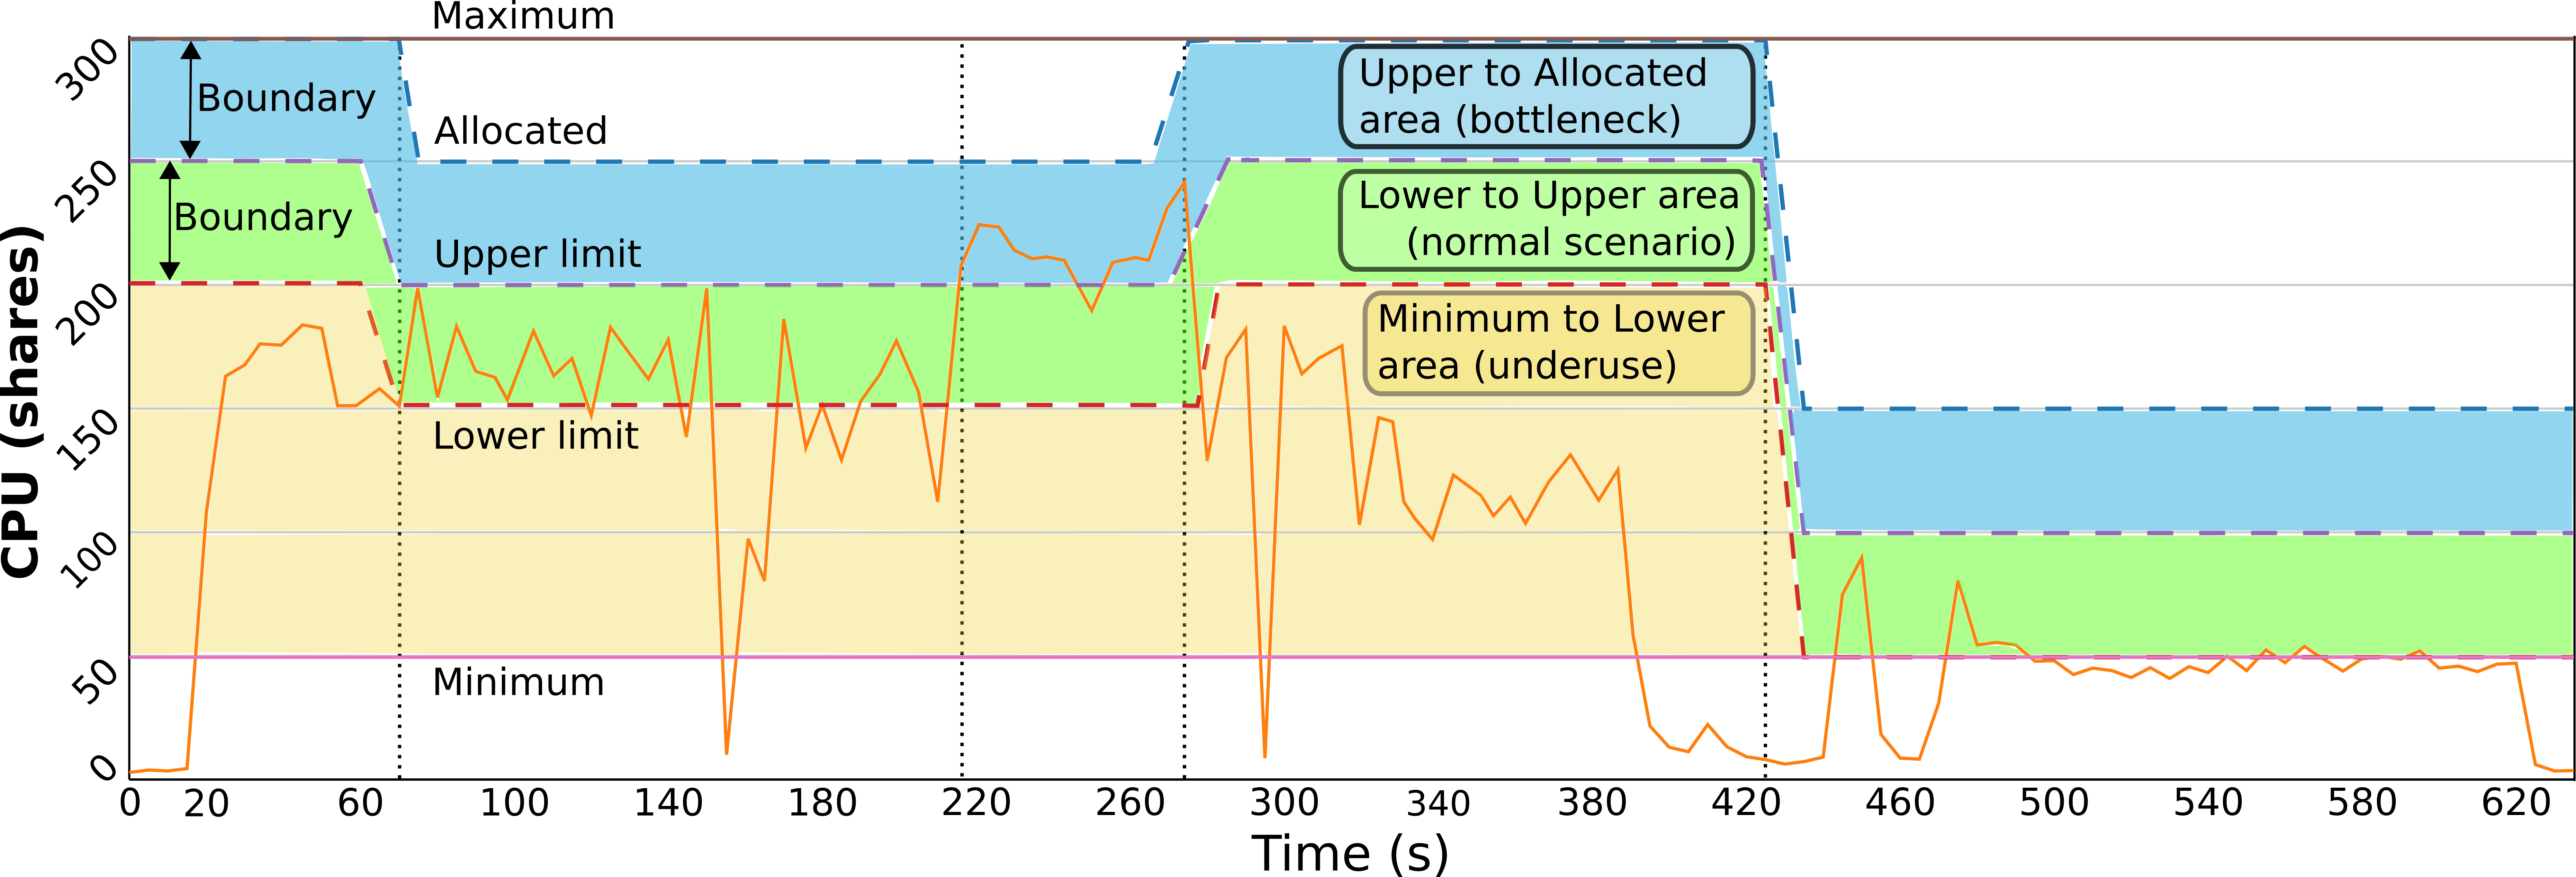
\includegraphics[width=0.99\textwidth]{../img/use_case/timeseries.png}
	\caption{Example showing scaling policies being applied}
	\label{fig:ScalingPolicy}
\end{figure}

\begin{itemize}
	\item \textbf{A time series} that varies (orange), this time series represents the container aggregated resource usage, in this case of the CPU.
	\item \textbf{Three varying thresholds} (dashed lines), which, from top to bottom, represent the allocated resource limit and the upper and lower boundaries (more on this later).
	\item \textbf{Three colored areas} (blue, green and ochre), which represent the areas between the previously mentioned thresholds.
	\item \textbf{Two horizontal lines} that do not vary, which represent the maximum and minimum resource limits. The maximum would be equivalent to the initial allocated resources on a traditional instance, while the minimum would represent the least amount of resources that we will grant the container.
\end{itemize}

As previously stated, the \textit{\textbf{Serverless Containers framework}} looks for a balance when it comes to setting an appropriate allocated resource amount, continuously responding to the resource usage variations. Such response can be seen in the several scaling operations that take place, such as at seconds 70 (down), 270 (up) and 420 (down). In order to detect the conditions that trigger these scaling requirements, two limits (or boundaries) are used.

\begin{itemize}
	\item \textbf{Upper limit}, which defines a threshold that, once surpassed, signals for a need to scale up the allocated resource limit to avoid any future bottleneck.
	\item \textbf{Lower limit}, which triggers a scale down of the allocated resource amount once the usage falls below the boundary.
\end{itemize}

Thus, it is easy to see that if the thresholds are considered, the first and third scaling operations were caused because the resource usage fell under the lower boundary, while the second was caused because it surpassed the upper boundary.

\subsection{Resource utilization}

It is interesting to note how important it is to keep a balance that does not impose a bottleneck but also stays close to the real resource usage. As previously stated, the serverless paradigm differs from the Cloud IaaS paradigm in that the resource limits can be modified multiple times over time, instead of just defining such limit once at the startup.

Moreover, if we consider that the user of a serverless platform typically does not specify such resource requirements and that the billed resources are only the used ones, the task of properly scaling and setting limits becomes a crucial one which falls to the provider.

Because of these reasons it is important to define a key ratio, the resource utilization, which can be easily obtained from the amount of used and the allocated resources. Figure~\ref{fig:ResourceUtilization} shows the previously used time window but with three areas as the focus of the study.

\begin{figure}[!tb]
	\centering
	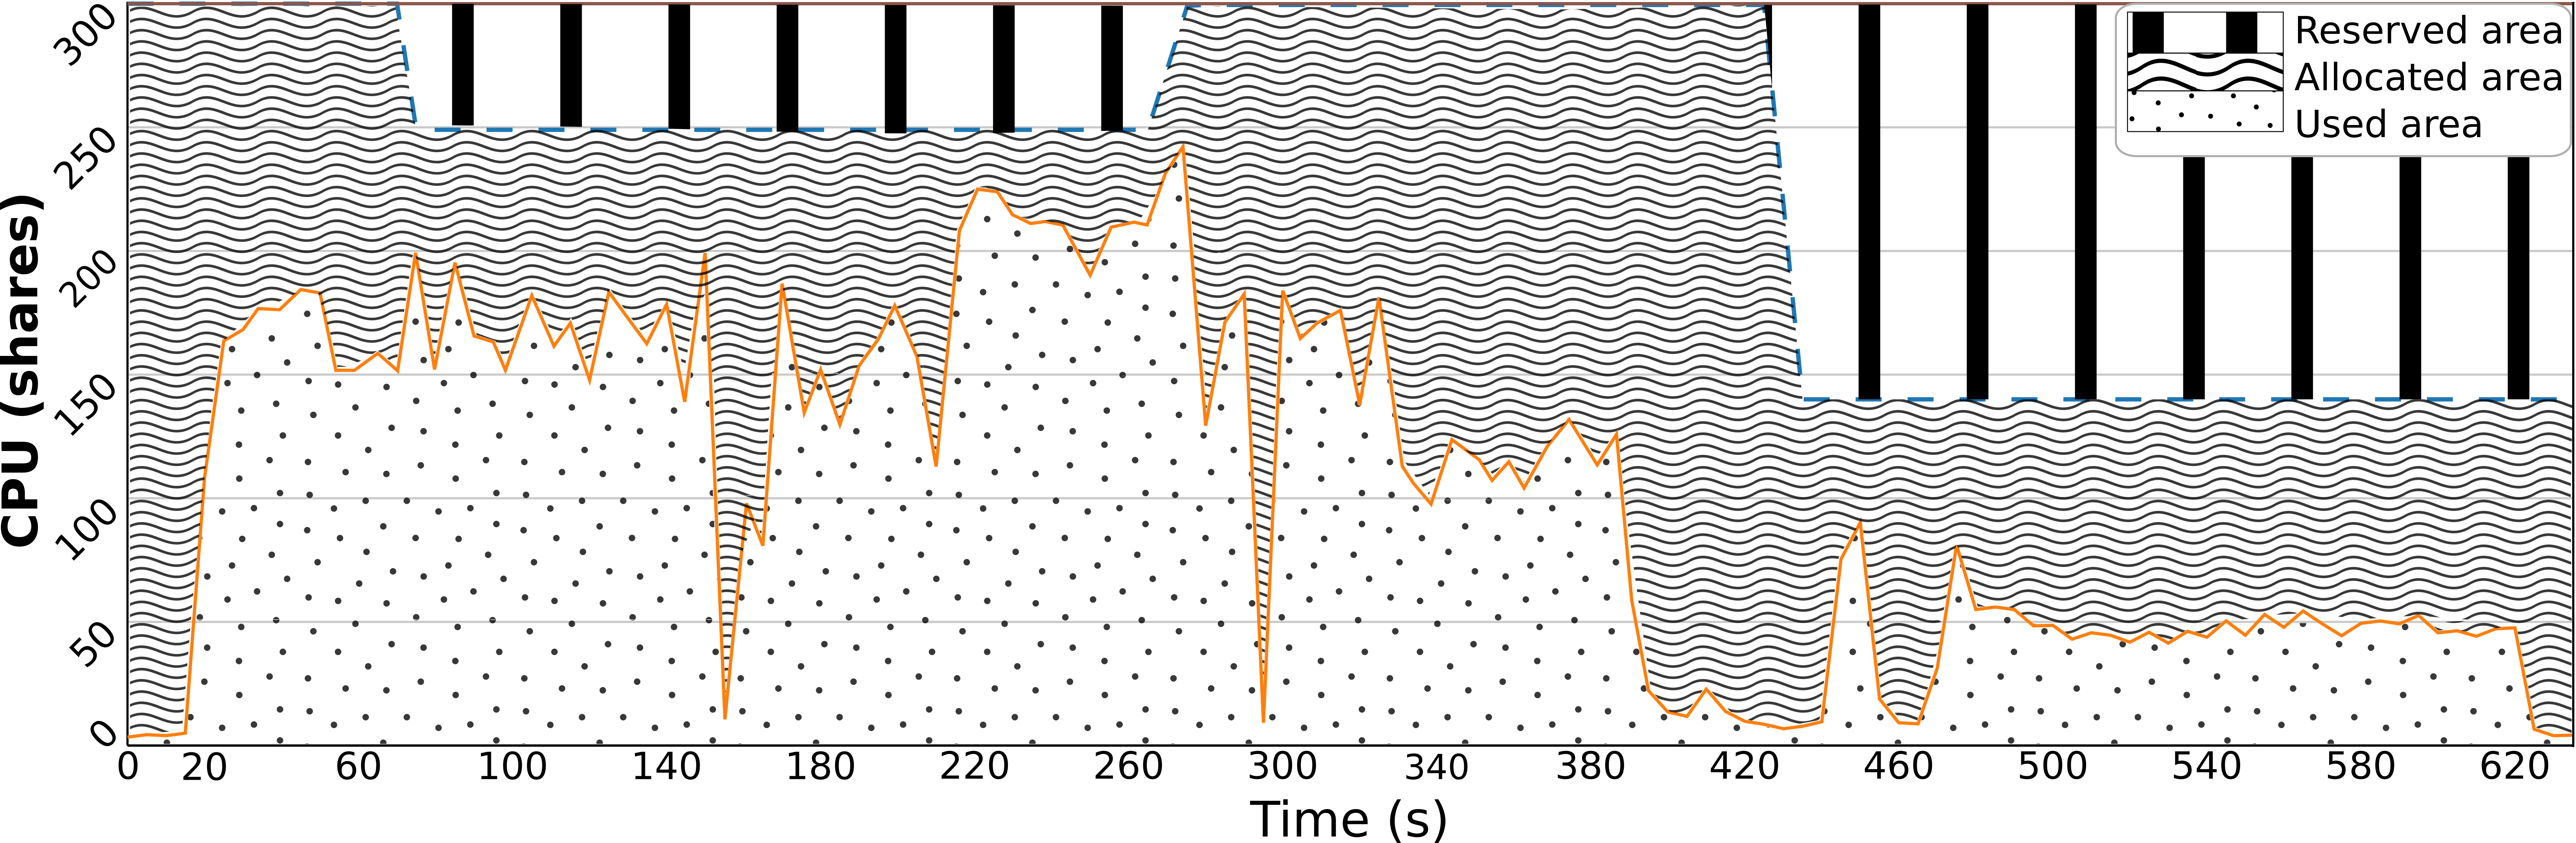
\includegraphics[width=0.99\textwidth]{../img/use_case/integrals.png}
	\caption{Example showing the resource utilization}
	\label{fig:ResourceUtilization}
\end{figure}

\begin{itemize}
	\item \textbf{Used area} (dots), which represents the amount of resources used by the container.
	\item \textbf{Allocated area} (waves), representing the changing amount of resources set apart for this container via the framework and a series of scaling operations.
	\item \textbf{Reserved area} (stripes), which represents the theoretical limit of resources that the container had at any moment. It is worth noting that this area would effectively represent the resource footprint of a virtual machine whose resources are allocated and never changed.
\end{itemize}

With these areas it is easy to see that the ratio of utilization of this serverless framework would be higher than the one achieved by a traditional instance. Moreover, an ideal serverless platform, which allocates only the strictly needed resources at any moment, performing instantaneous scaling operation, would have a ratio of 100\% (best-case scenario), while the ratio exposed by not performing any scaling operation, such as with the traditional instance, would be the worst-case scenario.

\section{Architecture}

\subsection{High-level diagram}

This framework has been designed using a microservice approach in order to ease its development as well as to create specialized units that can be reused or improved in isolation. In addition, by using this development technique it is also possible to implement a framework that inherently presents an internal parallelism that is useful when dealing with scenarios that require responsiveness, such as is the case with real-time and on-demand resource scaling. Figure~\ref{fig:HighLevelDiagram} shows a high-level diagram of the scenario on which the framework is deployed.

\begin{figure}[!tb]
	\centering
	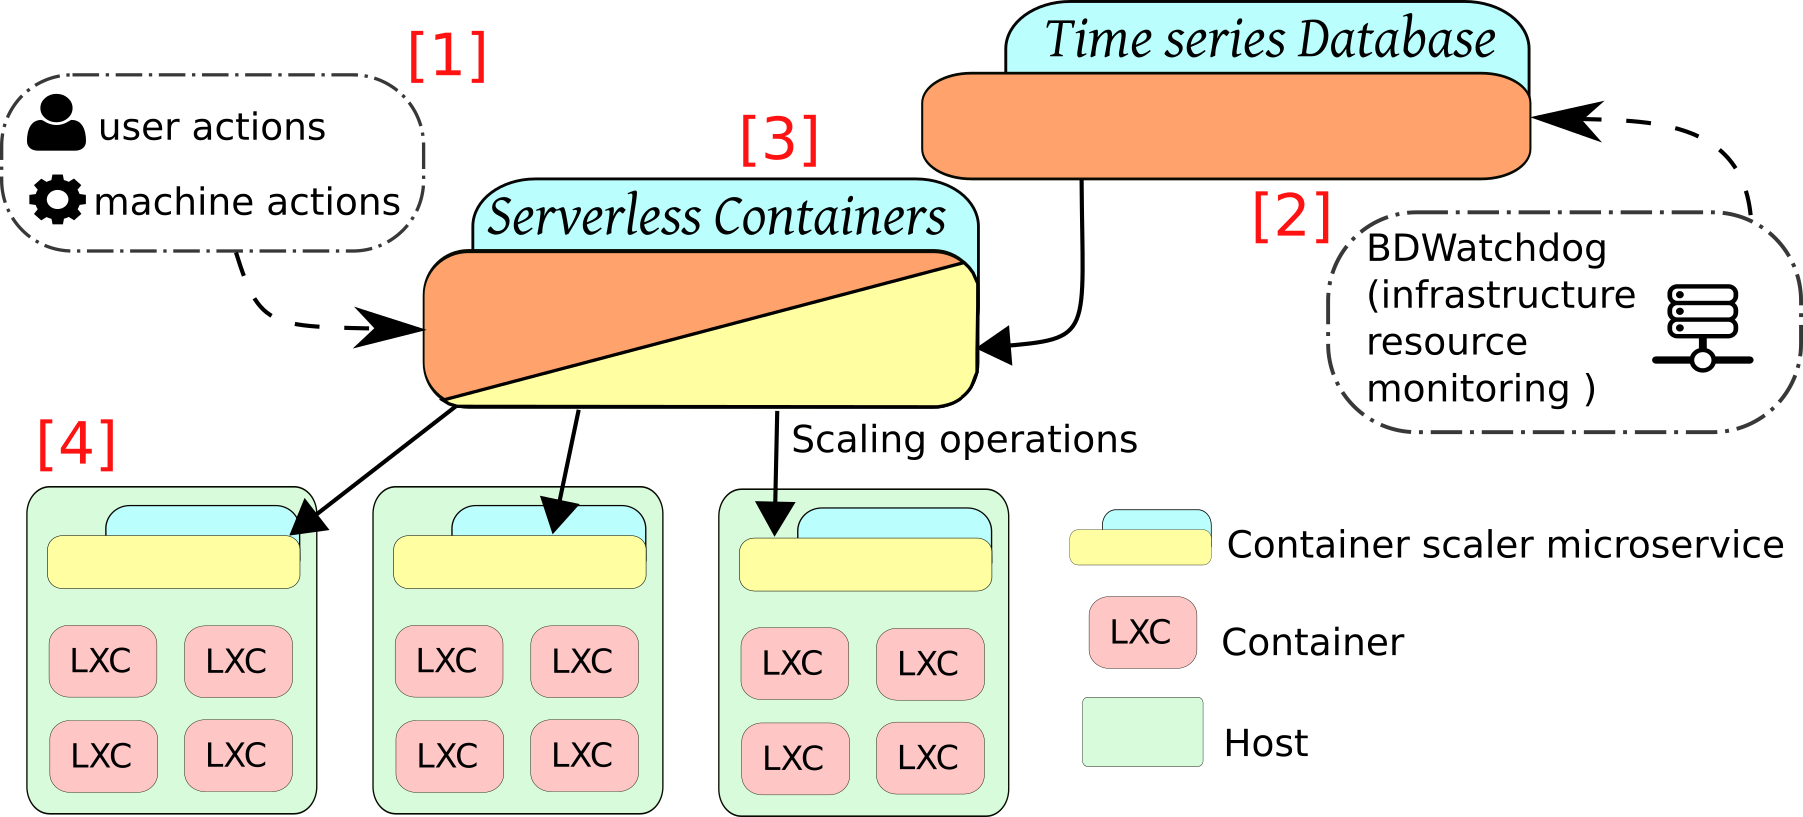
\includegraphics[width=0.99\textwidth]{../img/architecture/scenario_diagram.png}
	\caption{High-level Diagram}
	\label{fig:HighLevelDiagram}
\end{figure}

\begin{itemize}
	\item \textbf{[1]} Beginning with the framework's inputs, there are two: 1) the actions, that control the framework's behavior, both performed by an user or by another program through the API; and, 2) the resource monitoring time series, currently provided by an external framework (\textbf{\href{http://bdwatchdog.dec.udc.es/monitoring/index.html}{BDWatchdog}}), that are used in the policy decision for the resource scaling operations.
	
	\item \textbf{[2]} Continuing with the actual \textit{\textbf{Serverless Containers framework}}, which groups several microservices, some of which are placed on the controlled hosts. The microservices' inner workings are further specified on the following sections.
	
	\item \textbf{[3]} And finishing with the controlled infrastructure, which usually consists of several hosts running one or several containers each. Currently only the containers backed by the cgroups file system are supported by design and, more specifically, Linux Containers (LXC) have been used and thus have been proven to work with this framework.
\end{itemize}


\subsection{Microservice architecture}

As previously stated, the design followed to create the architecture of this framework uses several microservices that communicate and exchange information. Figure~\ref{fig:HighLevelMicroserviceLayout} shows a high-level diagram of the microservices layout.

\begin{figure}[!tb]
	\centering
	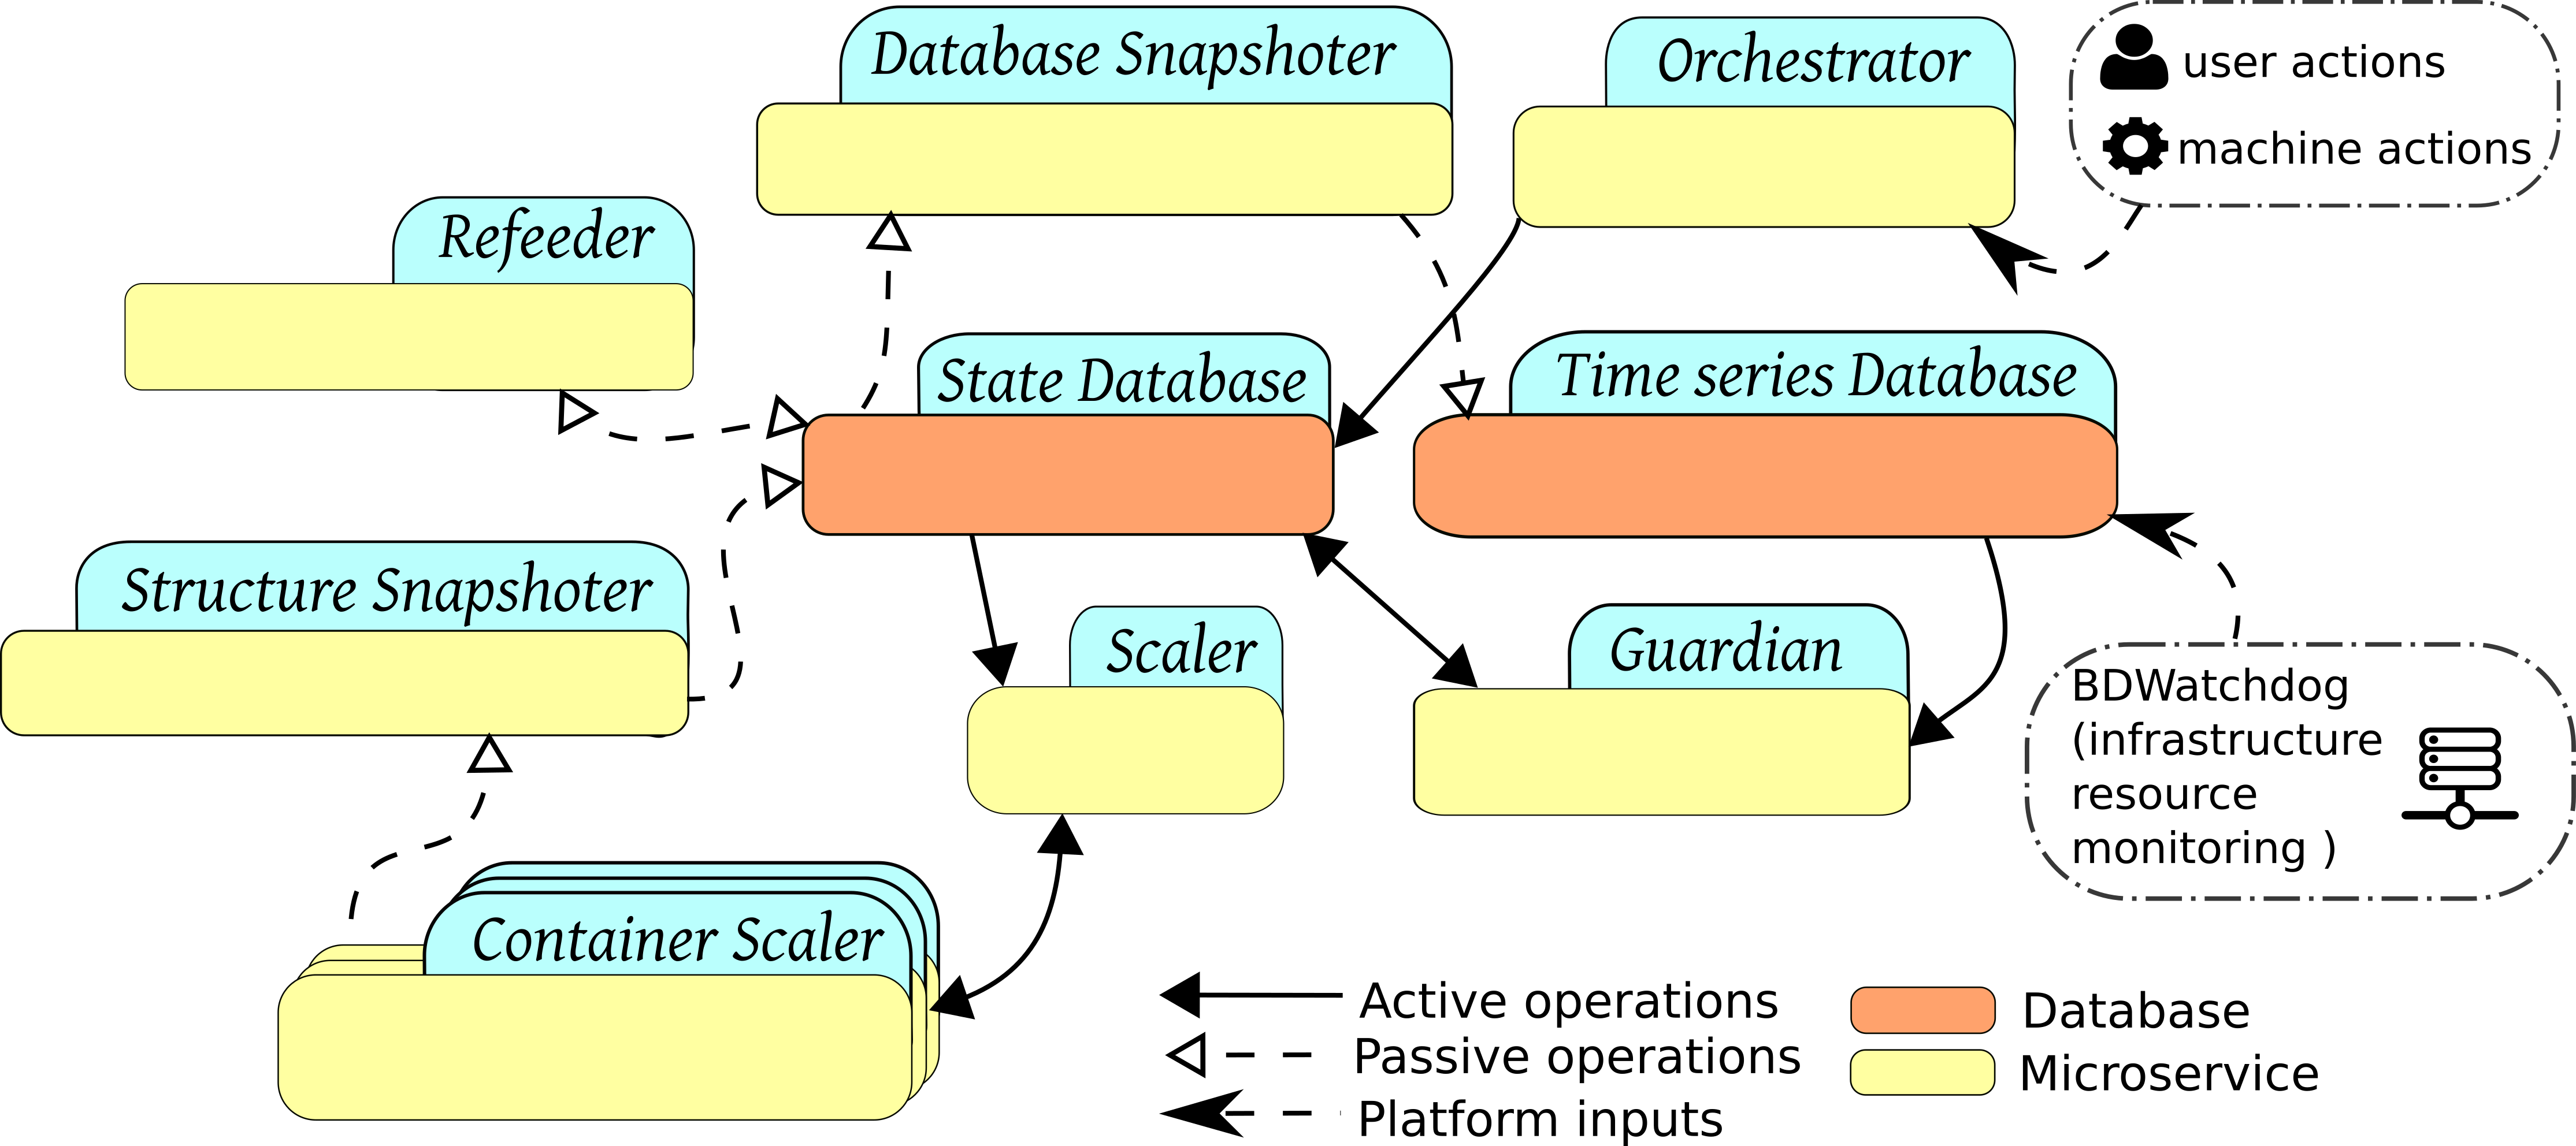
\includegraphics[width=0.99\textwidth]{../img/architecture/design_diagram.png}
	\caption{High-level Diagram}
	\label{fig:HighLevelMicroserviceLayout}
\end{figure}

As it can be seen, the microservices can be separated into active and passive ones, with the difference being that the passive ones focus on feedback operations to keep the framework continuously updated on the infrastructure's state, and the active ones, that use such information to change the state (the container's resource limits) accordingly and as needed.

\subsubsection{Passive Microservices}

The passive microservices (see Figure~\ref{fig:PassiveMicroservices}) are needed to continuously keep the central database (\textit{State Database}) updated with all the metadata that tracks the state of the infrastructure, from the number of containers and their thresholds to the allocated amounts of resources.

Some passive microservices are used to create aggregate data for entities such as applications (i.e., representing a group of containers) or to persist temporary information into a persistent database.

\begin{figure}[!tb]
	\centering
	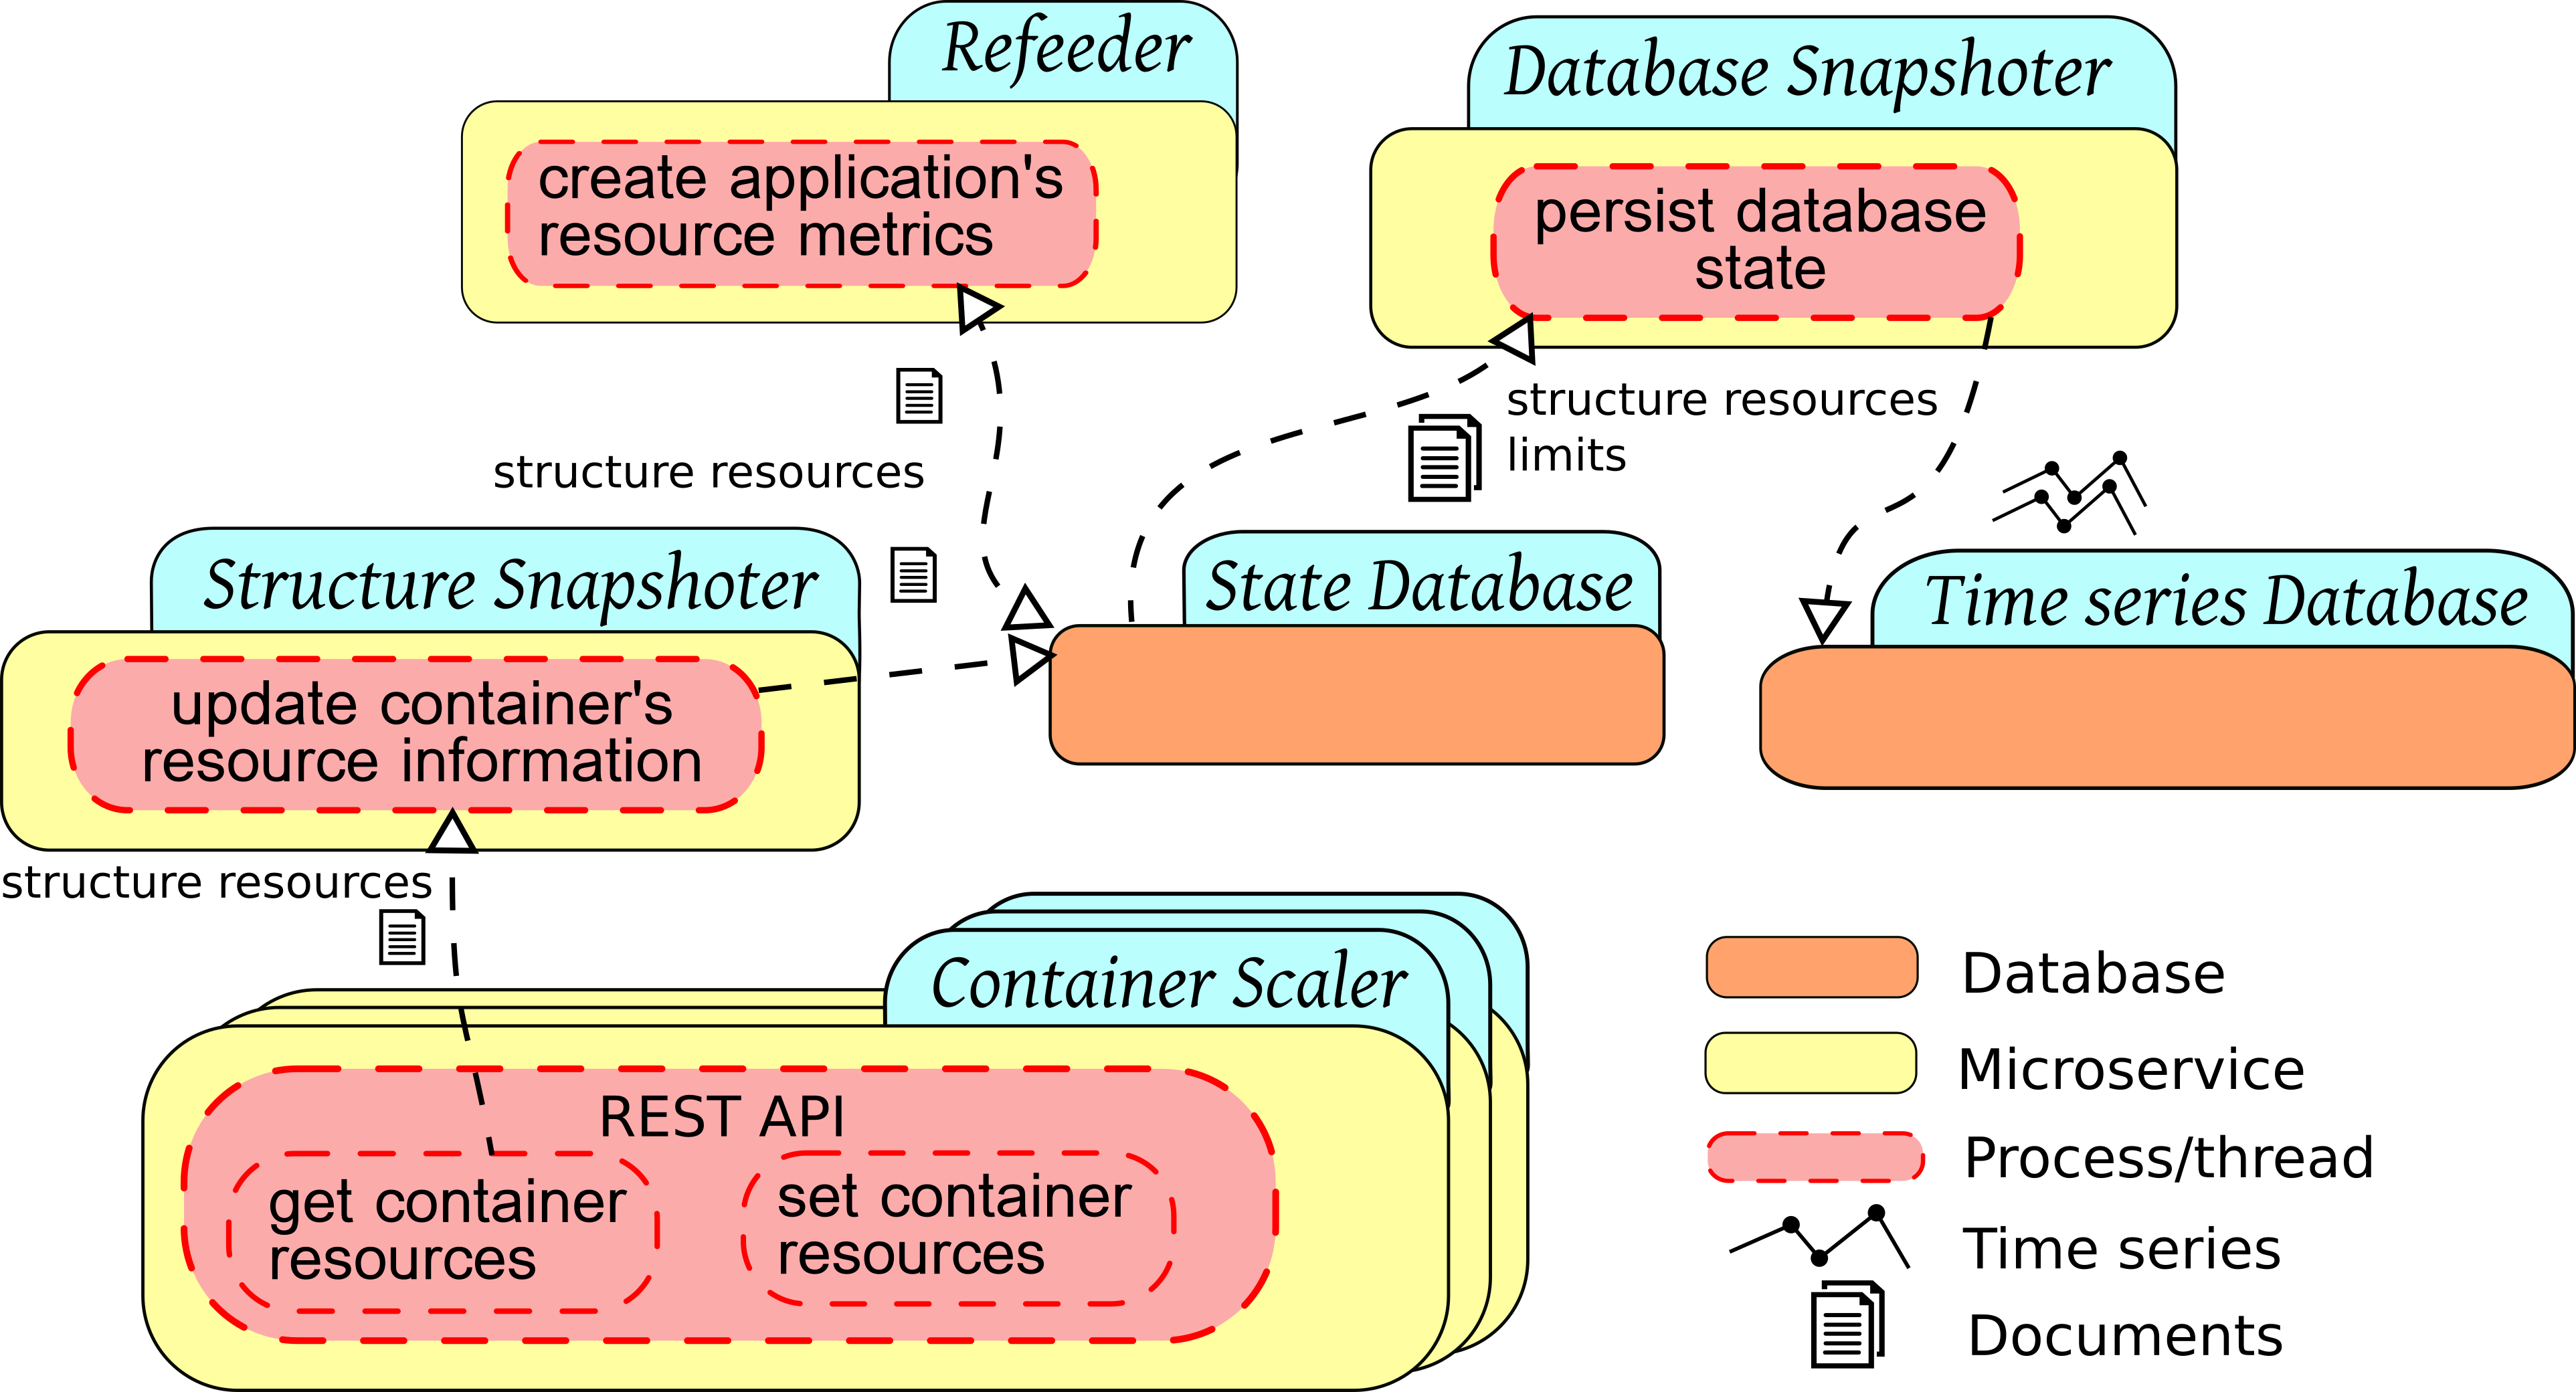
\includegraphics[width=0.99\textwidth]{../img/architecture/passive_services.png}
	\caption{Passive Microservices}
	\label{fig:PassiveMicroservices}
\end{figure}

\begin{itemize}
	\item \textbf{\textit{Structure Snapshoter}}: Continuously polls the actually applied limits of the containers and writes that information into the \textit{State Database}.
	\item \textbf{\textit{Database Snapshoter}}: Forwards the information temporarily stored on the \textit{State Database} to a persistent database, thus creating time series.
	\item \textbf{\textit{Refeeder Snapshoter}}: Aggregates and creates new metadata from existing one (e.g., allocated amount of CPU for an application composed of 3 containers).
\end{itemize}


\subsubsection{Active Microservices}

The active microservices (see Figure~\ref{fig:ActiveMicroservices}) are the actual ones that perform the scaling of the resources via changing the container resource limits on the underlying cgroups file system through a coordinated chain of events.

\begin{figure}[!tb]
	\centering
	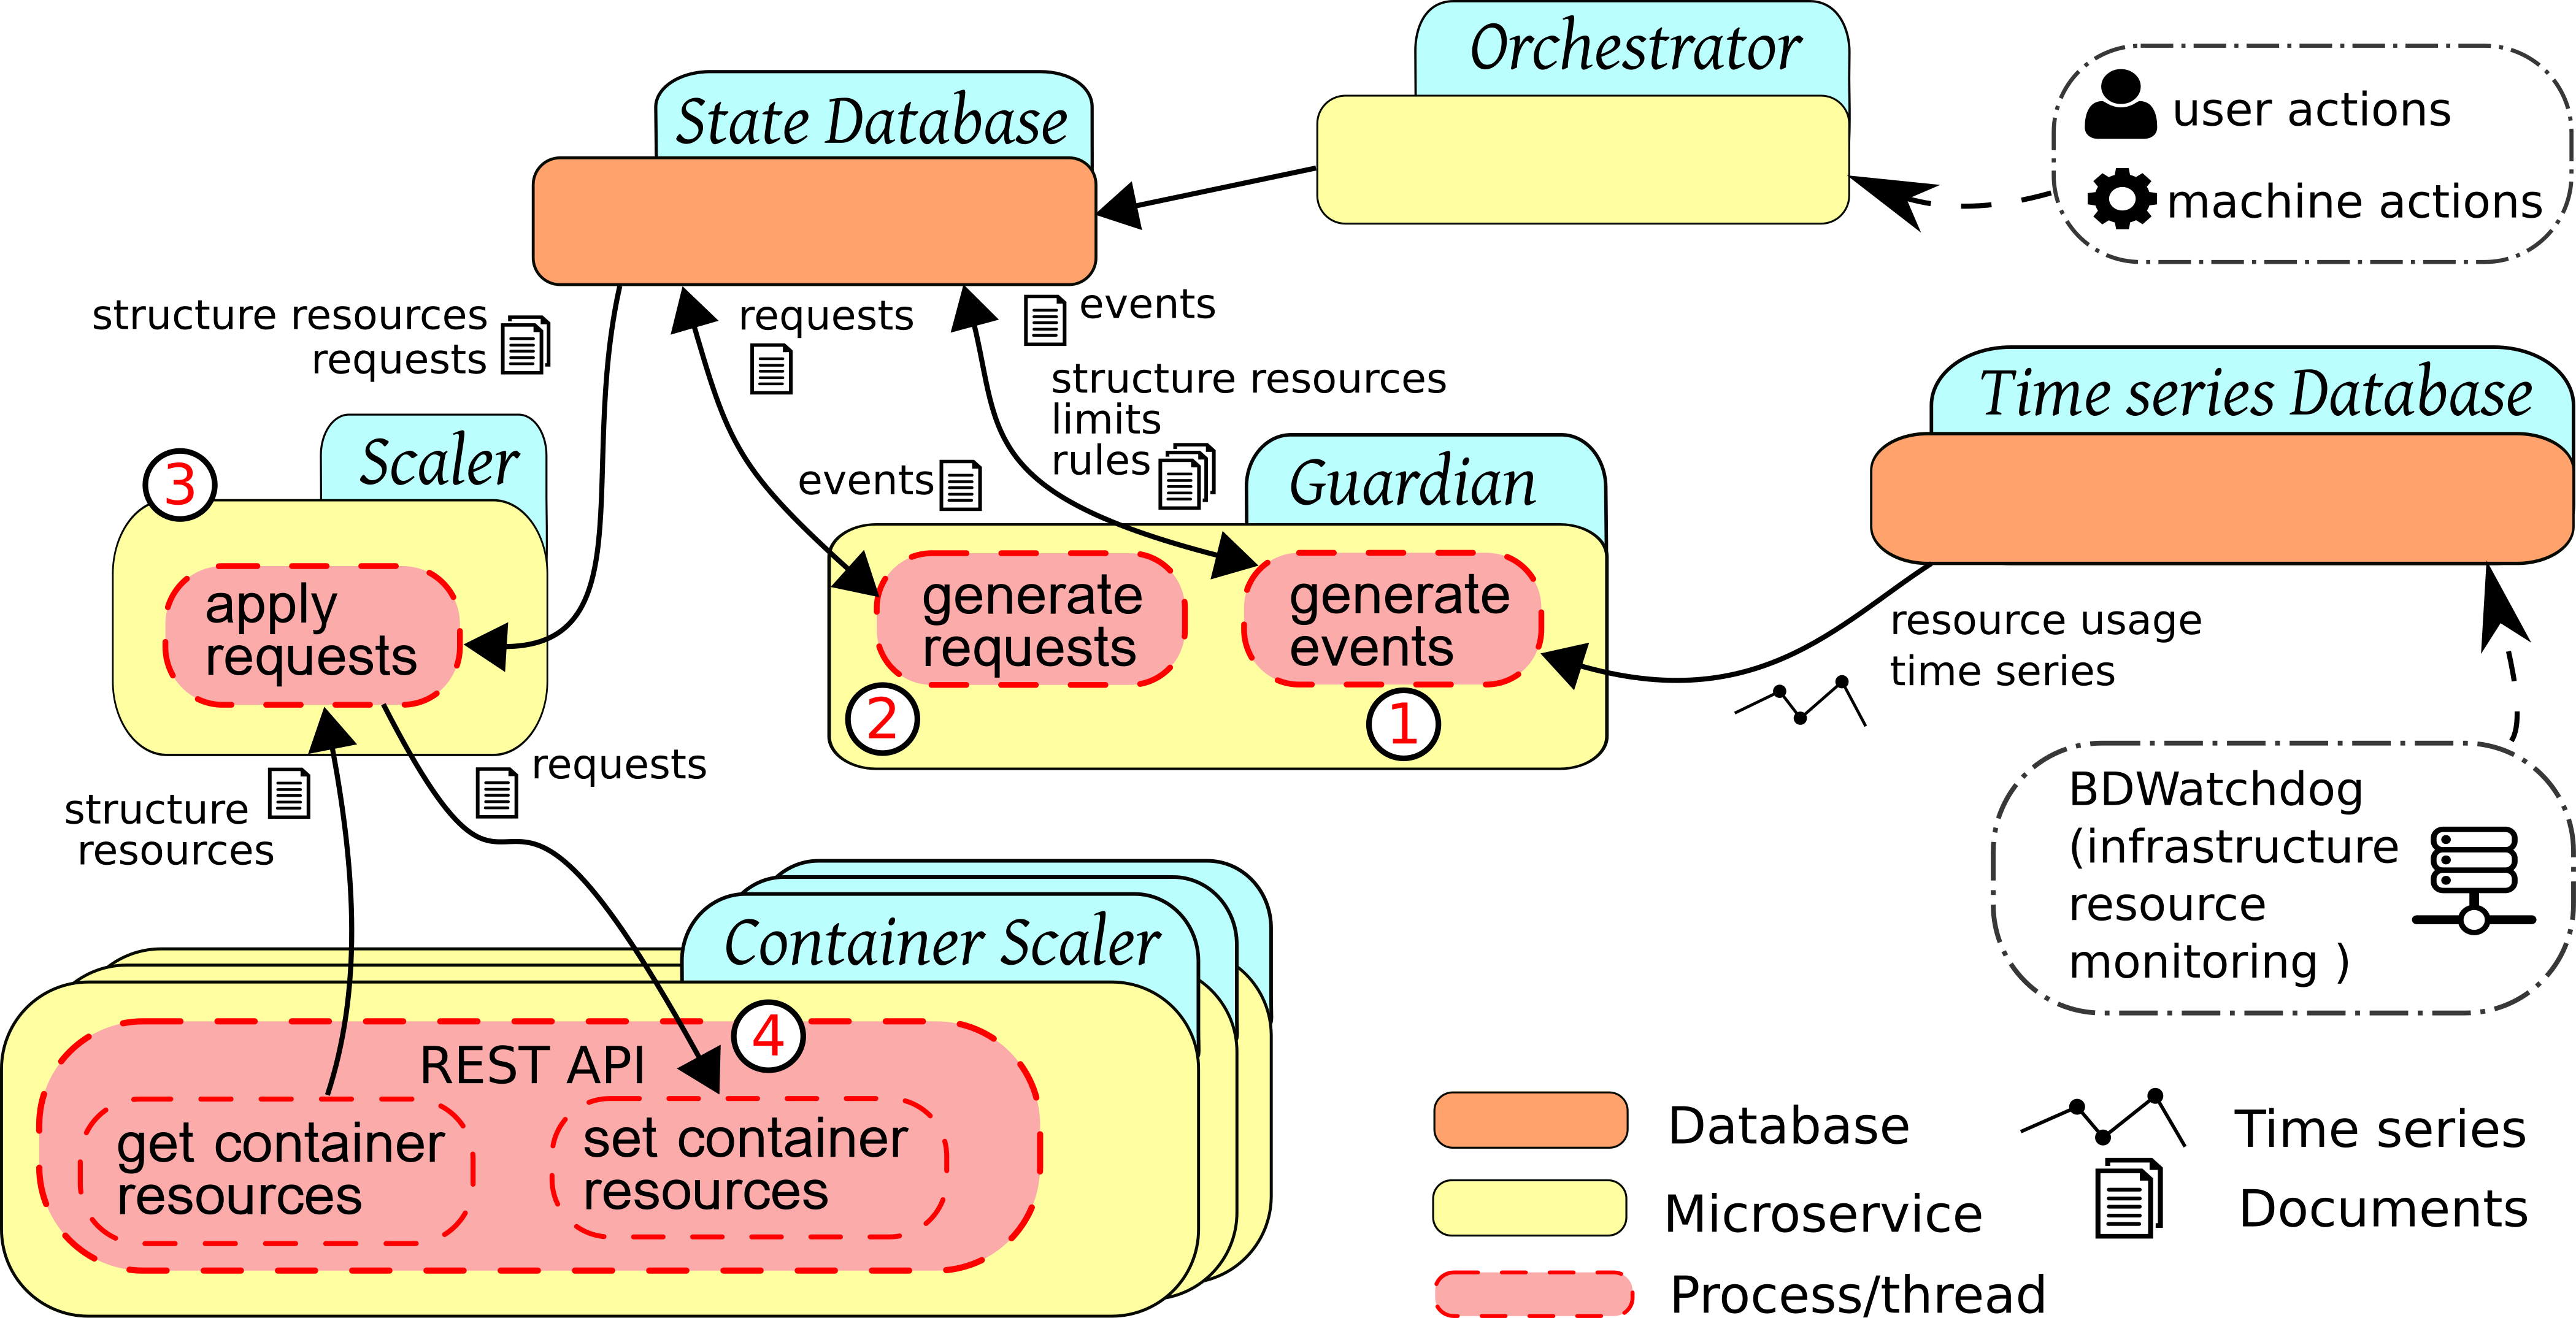
\includegraphics[width=0.99\textwidth]{../img/architecture/active_services.png}
	\caption{Active Microservices}
	\label{fig:ActiveMicroservices}
\end{figure}

As described on the Scaling policy subsection of the Use Case section~\ref{sec:UseCase}, in order to perform a scaling operation, the resource usage has to exceed the upper, or drop below the lower limit (see label 1 on Figure~\ref{fig:ActiveMicroservices}). After a configured time amount has passed on this state, the \textit{Guardian} microservice will create a scaling request (2) with the specific amount of resource to be changed. Such request will be picked up and processed by the \textit{Scaler} (3) and then, applied accordingly (4).

\begin{itemize}
	\item \textit{\textbf{Guardian}}: Working with time windows, it matches the real resource usages of the containers, as provided with the external resource monitoring, with the container limits stored on the \textit{State Database}. As a result of the matches it generates scaling requests.
	\item \textit{\textbf{Scaler}}: Polls the \textit{State Database} looking for requests to be applied to the containers.
\end{itemize}

\subsection{Other/Common Microservices and Databases}

Some microservices have an auxiliary role and are used both by active and passive microservices.
\begin{itemize}
	\item \textit{\textbf{Orchestrator}}: Exposes an API that can be used both by humans or scripts to configure the framework.
	\item \textit{\textbf{Container Scaler}}: This microservice has to be deployed on every infrastructure node whose hosted containers are to be scaled. This service is able to read and write the cgroups file system to perform the actual resource limit scaling operations.	
\end{itemize}


\section{Deployment}
\label{sec:Deployment}

The \textbf{\textit{Serverless Container framework}} can be deployed by cloning its GitHub repo and placing and starting the proper services, in the correct order and on the right environments.

To clone the project, you can use: \newline

\noindent \code{git clone https://github.com/UDC-GAC/ServerlessContainers} \newline

The actual deployment can be divided into different phases, as next described.

\subsection{Containers}

Serverless Containers supports any container engine and container technology that is backed by the cgroups file system. Specifically, for development the LXD container manager, which deploys Linux Containers (LXC), has been used.

There is no need for any specific configuration regarding the container deployment, nor there is a need to restart any container to begin adjusting its resources automatically. Nevertheless, in order to successfully perform such resource scaling operations, it may be needed to have permissions to write on the affected container's cgroups files. To do this, the \textit{Container Scaler} service has to be started with such permissions.

\subsection{Previous Requirements}

In order to work, \textbf{\textit{Serverless Containers}} needs to have a constant feed of the resources the containers are using, as close to real-time as possible in order to maintain the responsiveness of the scaling. This feature is currently provided by the  \textbf{\href{http://bdwatchdog.dec.udc.es/monitoring/index.html}{BDWatchdog}} framework, which is mainly composed of a time series database, \textbf{\href{http://opentsdb.net/}{OpenTSBD}} and of a resource monitor agent (atop) coupled with a processing pipeline which are able to work inside containers.

In addition, this framework has also at its core a JSON document database used as a cache of the system's state, referred to as \textit{State Database}. Currently, a \href{https://couchdb.apache.org/}{CouchDB} database is used. The installation of a functional CouchDB database is quite simple and there is no need for any specific configuration to be used by this frameworks. Nonetheless, because the need for a high response of the database operations, the fact that the stored data does not need to be persisted across time and that the required storage size is relatively small (no more than 1 GiB for 30+ containers), it may be desirable to use it with an in-memory storage file system.

Finally, other requirements include the Python3 runtime environment and other Python packages such as Flask.

\subsection{Microservices}

All of the microservices deployed by \textbf{\textit{Serverless Containers}} have been implemented as Python3 programs and thus, can be started by simply launching them with the system's interpreter. In addition, most of them also interact with the \textit{State Database} so it is advisable that their latency with the latter is small. Other latencies that may be interesting to take into account, as well as a proposed placement, are shown in Figure~\ref{fig:MicroservicePlacement}.

\begin{figure}[!tb]
	\centering
	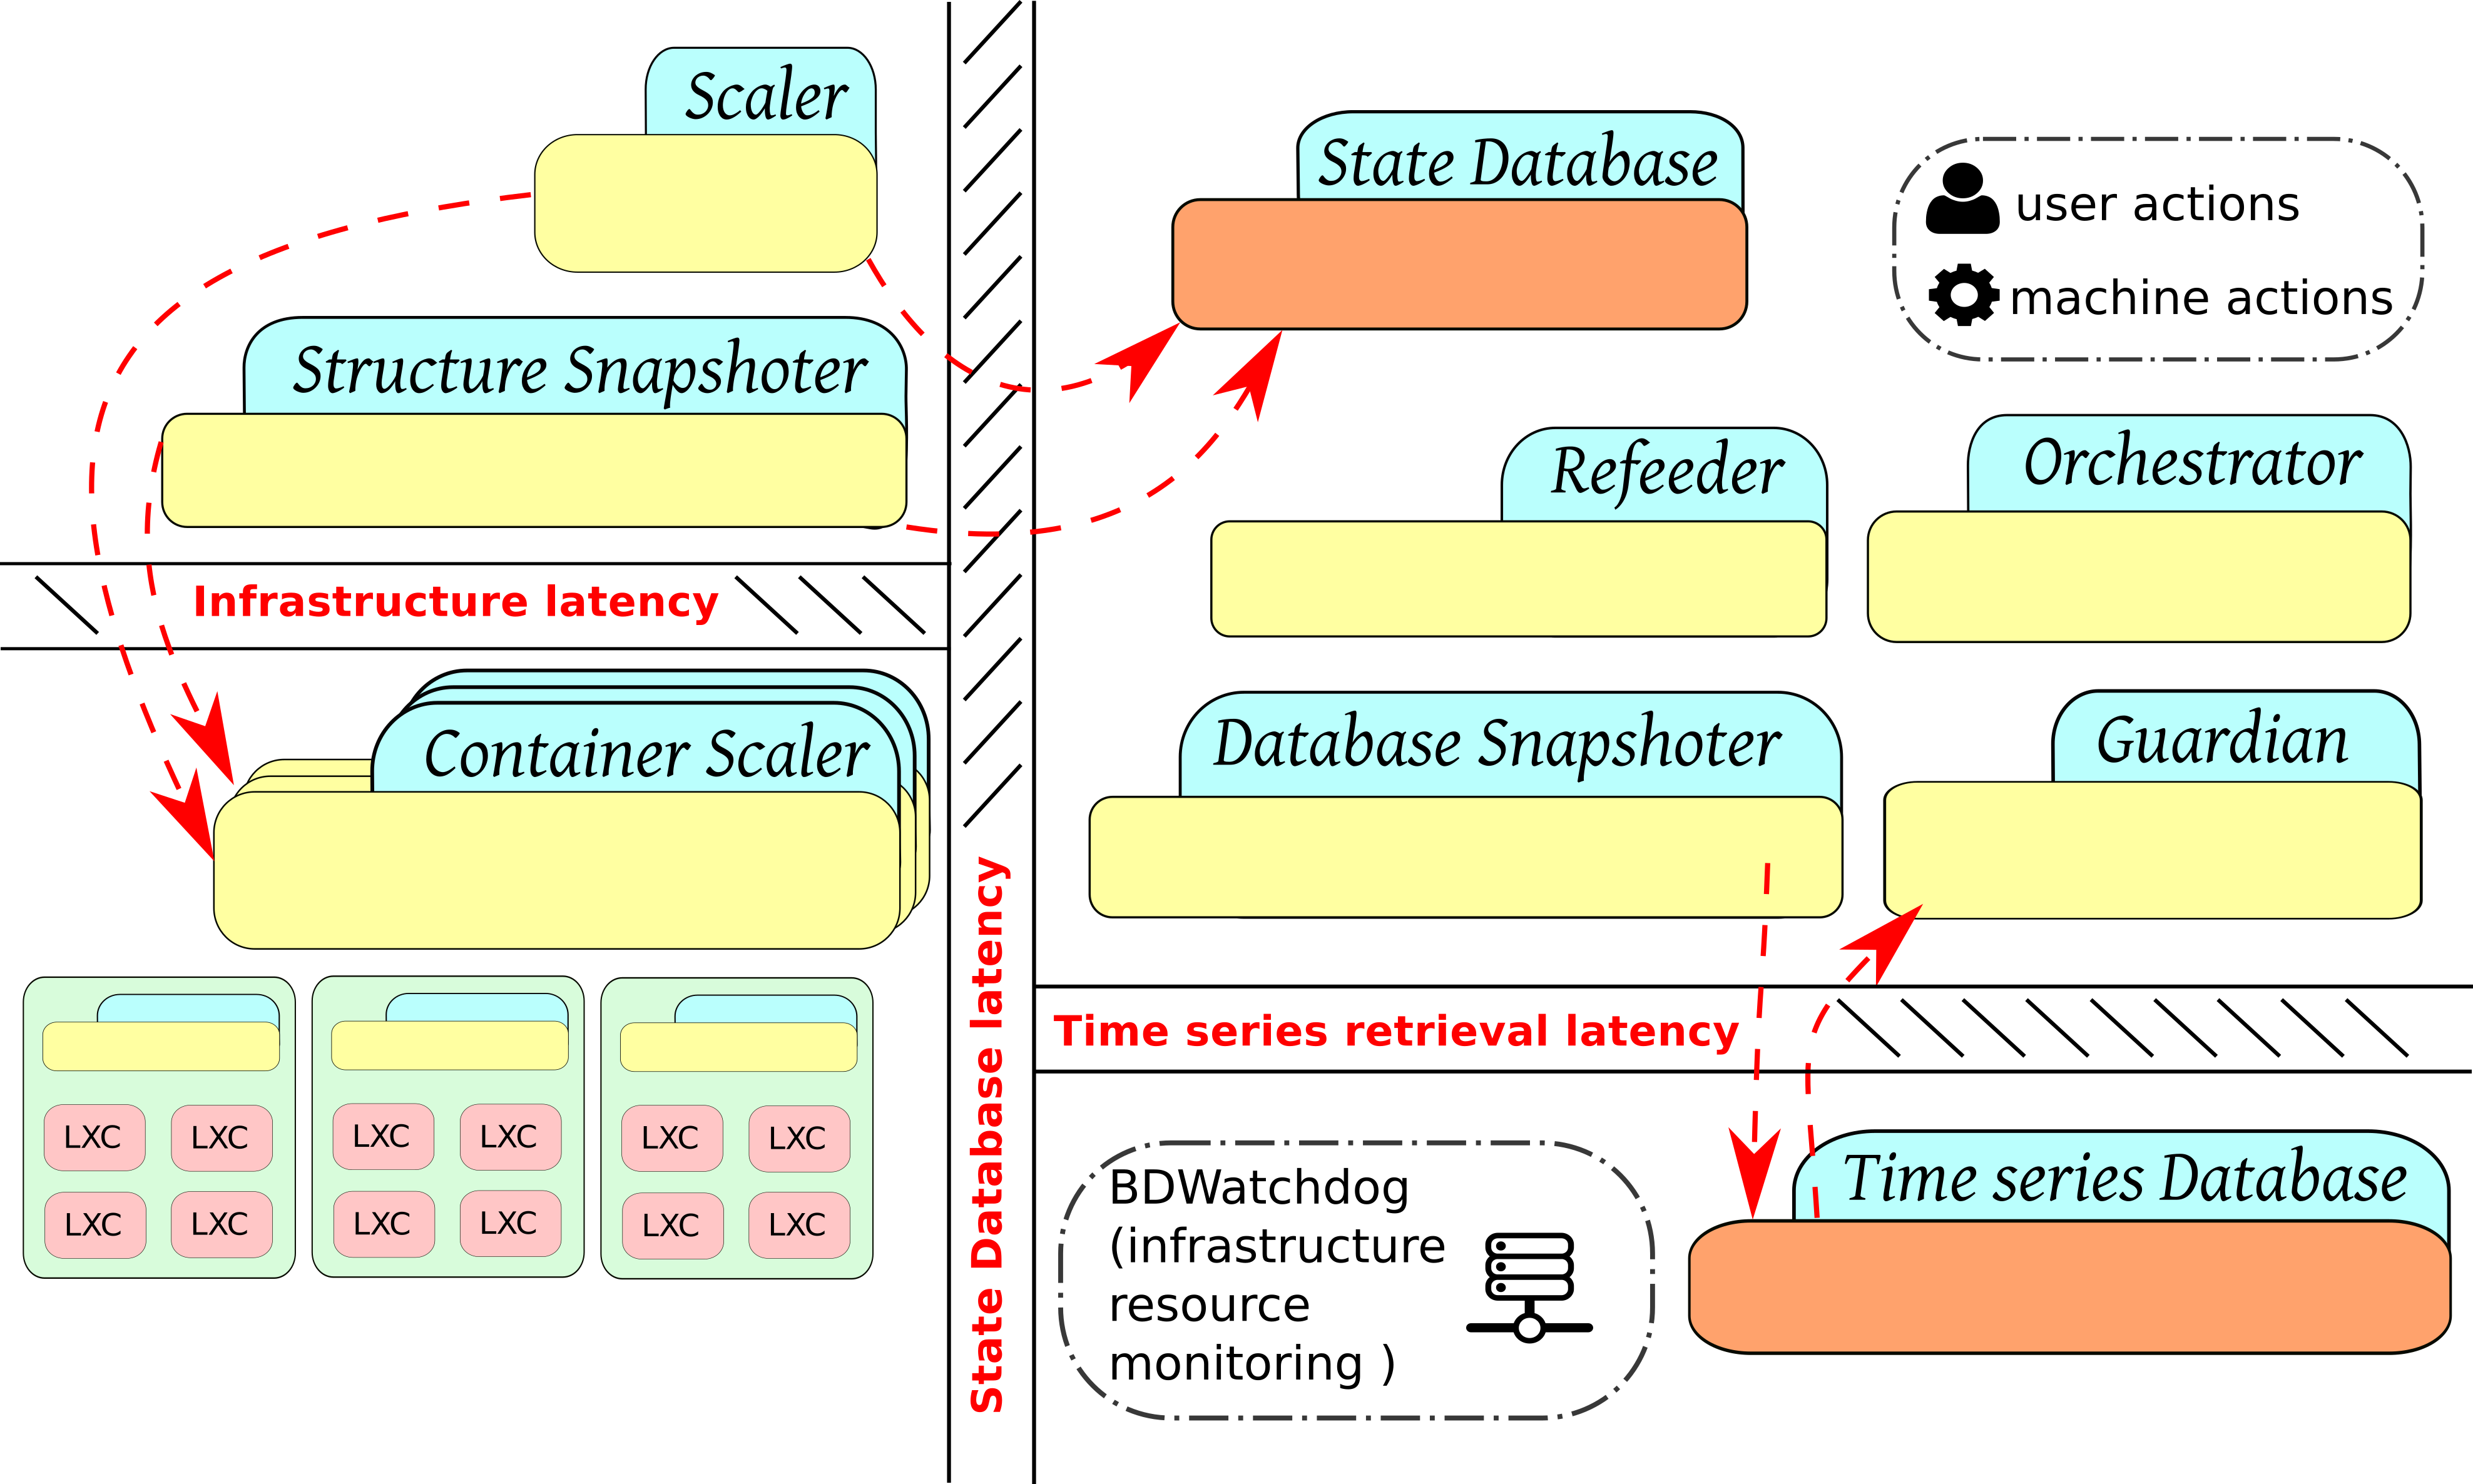
\includegraphics[width=0.99\textwidth]{../img/deployment/placement.png}
	\caption{Microservice placement}
	\label{fig:MicroservicePlacement}
\end{figure}

Finally, it should also be considered that some of these microservices, due to their inner operations and continuous polling, can present an overhead that although should not be particularly high, it could be noticeable particularly in experimentation testbeds. Because of this, it is advisable to run as many microservices as possible in an dedicated/isolated instance separated from any environment not to be disturbed.

\subsubsection{Passive}

Services: \textbf{\textit{Structure Snapshoter}}, \textbf{\textit{Database Snapshoter}}, \textbf{\textit{Refeeder Snapshoter}}

Regarding the passive microservices, the \textit{Structure Snapshoter} in particular has to poll the containers via the \textit{Container Scaler} service, which is deployed in all the infrastructure hosts that run containers. Because of this, the latency of this microservice should also be small when interacting with the nodes.

\subsubsection{Active}

Services: \textbf{\textit{Guardian}}, \textbf{\textit{Scaler}}

As with the \textit{Structure Snapshoter} passive microservice, the \textit{Scaler} also need to interact with the infrastructure HOSTS and their \textit{Container Scaler} service, so the latency between the two should be kept low.


\subsubsection{Other}

Services: \textbf{\textit{Orchestrator}}, \textbf{\textit{Container Scaler}}

When it comes to the remaining microservices, the \textit{Orchestrator} should be placed near the \textit{State Database}, as it may require to perform many database operations in a short amount of time, while the \textit{Container Scaler} is required to be deployed on each infrastructure host that runs containers.

\section{Quickstart}

The \textbf{\textit{Serverless Container framework}} has been developed to be modular at its core, meaning that it can be scaled and adapted to the number of hosts and containers present in the infrastructure, from a few containers on a single host to dozens of containers spanned across multiple hosts.

In order to show a quickstart with an example of usage, and keep it simple, this scenario will use 2 containers deployed on 1 host, with CPU as the only scaled resource. We will also consider LXD as the technology used to deploy the containers, that the host `host0' is network-reachable using such name, and that a CouchDB database is running and accessible as `couchdb'. It is also required to have resource monitoring and a time series database.


\subsection{Container Scaler deployment}

First, in order to make sure that the containers are properly detected and supported, we have to make sure that the \textit{Container Scaler} service (deployed on every host) is running.

To do so, we can deploy 2 containers using LXD (in this case spawning an Ubuntu 20.04 distro): \newline

\noindent \code{lxc init ubuntu:20.04 cont0} \newline
\code{lxc init ubuntu:20.04 cont1} \newline
\code{lxc start cont0 cont1} \newline

Next, from the framework's folder, start the service: \newline

\noindent \code{bash scripts/services/start\_node\_rescaler.sh} \newline


\begin{figure}[!tb]
	\centering
	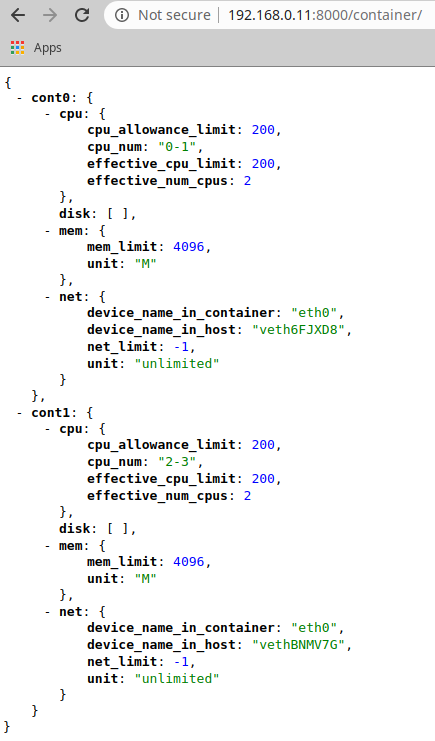
\includegraphics[width=0.59\textwidth]{../img/quickstart/ContainerScaler.png}
	\caption{\textit{Container Scaler} API output}
	\label{fig:ContainerScalerAPI}
\end{figure}

To make sure that the containers are accessible to the service, you can open a web browser and point to the host's IP and the `8000' port and `/container' path. You should see something similar to Figure~\ref{fig:ContainerScalerAPI}. As you can see, the memory, disks and network resources are also reported, but they will be ignored on this guide.


\subsection{Initializing the container's limit}
As of now, the containers could have no limits applied (-1 value) or some predefined limits. Such resource limits can be easily changed through REST API calls to the \textit{Container Scaler} service. We can do this with the `curl' command inside the scripts of the NodeRescaler folder.\newline

\noindent \code{curl -X PUT -H "Content-Type: application/json" \textbackslash } \newline
\code{-d '\{"cpu": \{"cpu\_allowance\_limit": "200","cpu\_num": "0,1"\}\}' \textbackslash } \newline
\code{http://host0:8000/container/cont0} \newline
\newline
\noindent \code{curl -X PUT -H "Content-Type: application/json" \textbackslash } \newline
\code{-d '\{"cpu": \{"cpu\_allowance\_limit": "200","cpu\_num": "2,3"\}\}' \textbackslash } \newline
\code{http://host0:8000/container/cont1} \newline

However, it has to be note that this out-of-band limit changing operation is only intended for initializations or hard and direct limit changes for experimentation reasons, for example.


\subsection{Initializing State Database}

In order to continue with the guide, and before initializing the remaining microservices, we have to initialize the \textit{State Database}. This is needed considering that the services are configured and tuned via unique documents stored on such \textit{State Database}. This allows to change their configuration on-the-fly. To perform this initialization, you can use Python scripts that connect to the database and insert the proper documents, as pre-configured by the user.

To initialize the services with their respective configuration files: \newline

\noindent \code{python3 quickstart/StateDatabase/services.py} \newline

To initialize the rules that will govern the rescaling policies, as well as the events and requests databases, run: \newline

\noindent \code{python3 quickstart/StateDatabase/events\_and\_requests.py} \newline
\code{python3 quickstart/StateDatabase/rules.py} \newline

Finally, in order to initialize the containers and the hosts, as well as the container's limit thresholds, run: \newline

\noindent \code{python3 quickstart/StateDatabase/limits} \newline
\code{python3 quickstart/StateDatabase/structures.py} \newline

\subsection{Start the Orchestrator}

In order to check that the previous step finished correctly and that all of the necessary documents were stored on the \textit{State Database}, you can use the \textit{Orchestrator} service as it exposes an API of the database contents. Start it with: \newline

\noindent \code{bash scripts/services/start\_orchestrator.sh} \newline

And then check its output by opening a browser with the instance's IP on which the \textit{Orchestrator} was started, the port `5000' and the path `/structure/cont0' (to see the cont0 structure document). You should see something similar to Figure~\ref{fig:OrchestratorAPI}.

\begin{figure}[!tb]
	\centering
	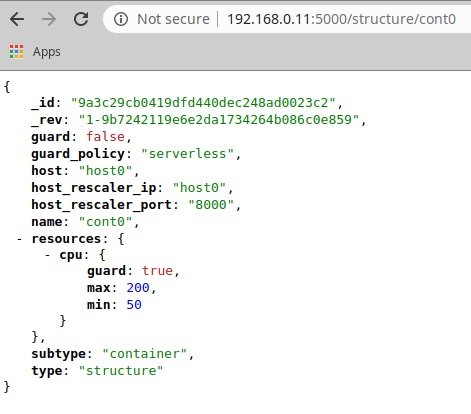
\includegraphics[width=0.99\textwidth]{../img/quickstart/OrchestratorCont0.png}
	\caption{\textit{Orchestrator} API output of container 0}
	\label{fig:OrchestratorAPI}
\end{figure}

As you can see, the container is registered with resource limits of 50 and 200 for the minimum and maximum values, respectively. It can also be appreciated that its configuration marks it as a non-scalable container (i.e., guard:false), even though the CPU is marked as subjected to be scaled.

The full \textit{Orchestrator} API can be checked below and it can be used via scripts that perform REST calls. Using this service and the scripts, we will make sure that both of the containers are set to be left unscaled (unguarded): \newline

\noindent \code{bash scripts/Orchestrator/Structures/set\_to\_unguarded.sh cont0} \newline
\code{bash scripts/Orchestrator/Structures/set\_to\_unguarded.sh cont1} \newline

A return code of 201 ensures that the operation was carried out correctly.

\subsection{Starting the services}

Now that the containers are up and running and that the \textit{State Database} has been initialized, the remaining microservices can also be started. First, the passive services should be started (tmux is used to de-attach the program from the terminal and keep the service running): \newline

\noindent \code{tmux new -d -s "DatabaseSnapshoter" "python3 src/Snapshoters/DatabaseSnapshoter.py"} \newline
\code{tmux new -d -s "StructureSnapshoter" "python3 src/Snapshoters/StructuresSnapshoter.py"} \newline

Both of these services show an output each time they finish a polling operation. The polling time can be configured with their respective configuration documents. Secondly, the active services can be started: \newline

\noindent \code{tmux new -d -s "Guardian" "python3 src/Guardian/Guardian.py"} \newline
\code{tmux new -d -s "Scaler" "python3 src/Rescaler/ClusterScaler.py"} \newline

These services also output what they are doing, processing time windows with a time length that is configurable.

At this point, all of the necessary services would be running, however, nothing would be happening as both of the containers are in an `unguarded' state, that is, they are being left untouched. We will also deactivate the \textit{Scaler} service for now: \newline

\noindent \code{curl -s -X PUT -H "Content-Type:application/json" \textbackslash} \newline \code{http://orchestrator:5000/service/scaler/ACTIVE -d `\{"value":"false"\}'}


\subsection{Transitioning the containers to serverless instances}

In order to move the containers from following the resource management of a traditional instance, that is, having the initial resources fixed throughout their life-cycle, into a serverless environment, we can use the same scripts as before: \newline

\noindent \code{bash scripts/Orchestrator/Structures/set\_to\_guarded.sh cont0} \newline
\code{bash scripts/Orchestrator/Structures/set\_to\_guarded.sh cont1} \newline

Now, both container are being monitored by the \textit{Guardian} service and their CPU limits will be scaled according to their internal CPU usage. However, the \textit{Guardian} service will only create Requests for resource scaling, either to lower or increase them, but not actual changes will be made to the resource's limits. In order to apply the Requests as generated by the \textit{Guardian} service, we will have to rely on the \textit{Scaler} service. To let it work, we will now activate it: \newline

\noindent \code{curl -s -X PUT -H "Content-Type:application/json" \textbackslash} \newline \code{http://orchestrator:5000/service/scaler/ACTIVE -d '{"value":"true"}'} \newline

Now, with all of the services properly working, the serverless environment should be fully functional for the containers. As seen in Figure~\ref{fig:ContainerScalingExample}, a serverless policy is being applied to the container as its resources are being continuously modified according to the resource usage:
\begin{itemize}
	\item \textbf{1)} In the beginning, the CPU is idle so that after enough time passes with the CPU underused, a scaling down operation is performed.
	\item \textbf{2)} Later, the CPU is suddenly heavily used to the point that a bottleneck occurs. To fix this, a scaling up operation is performed.
	\item \textbf{3)} However, after increasing the resources, the upscale operations gave too many resources and now there is another under-utilization scenario. A second scaling down operation is performed to adjust them.
	\item \textbf{4)} The usage fits perfectly between the lower and upper limits so it is under control.
	\item \textbf{5)} Finally, the CPU is idle again so that a last scaling down operation is carried out, leaving the allocated resources to the theoretical minimum (minimum + 2 x boundary).
\end{itemize}

\begin{figure}[!tb]
	\centering
	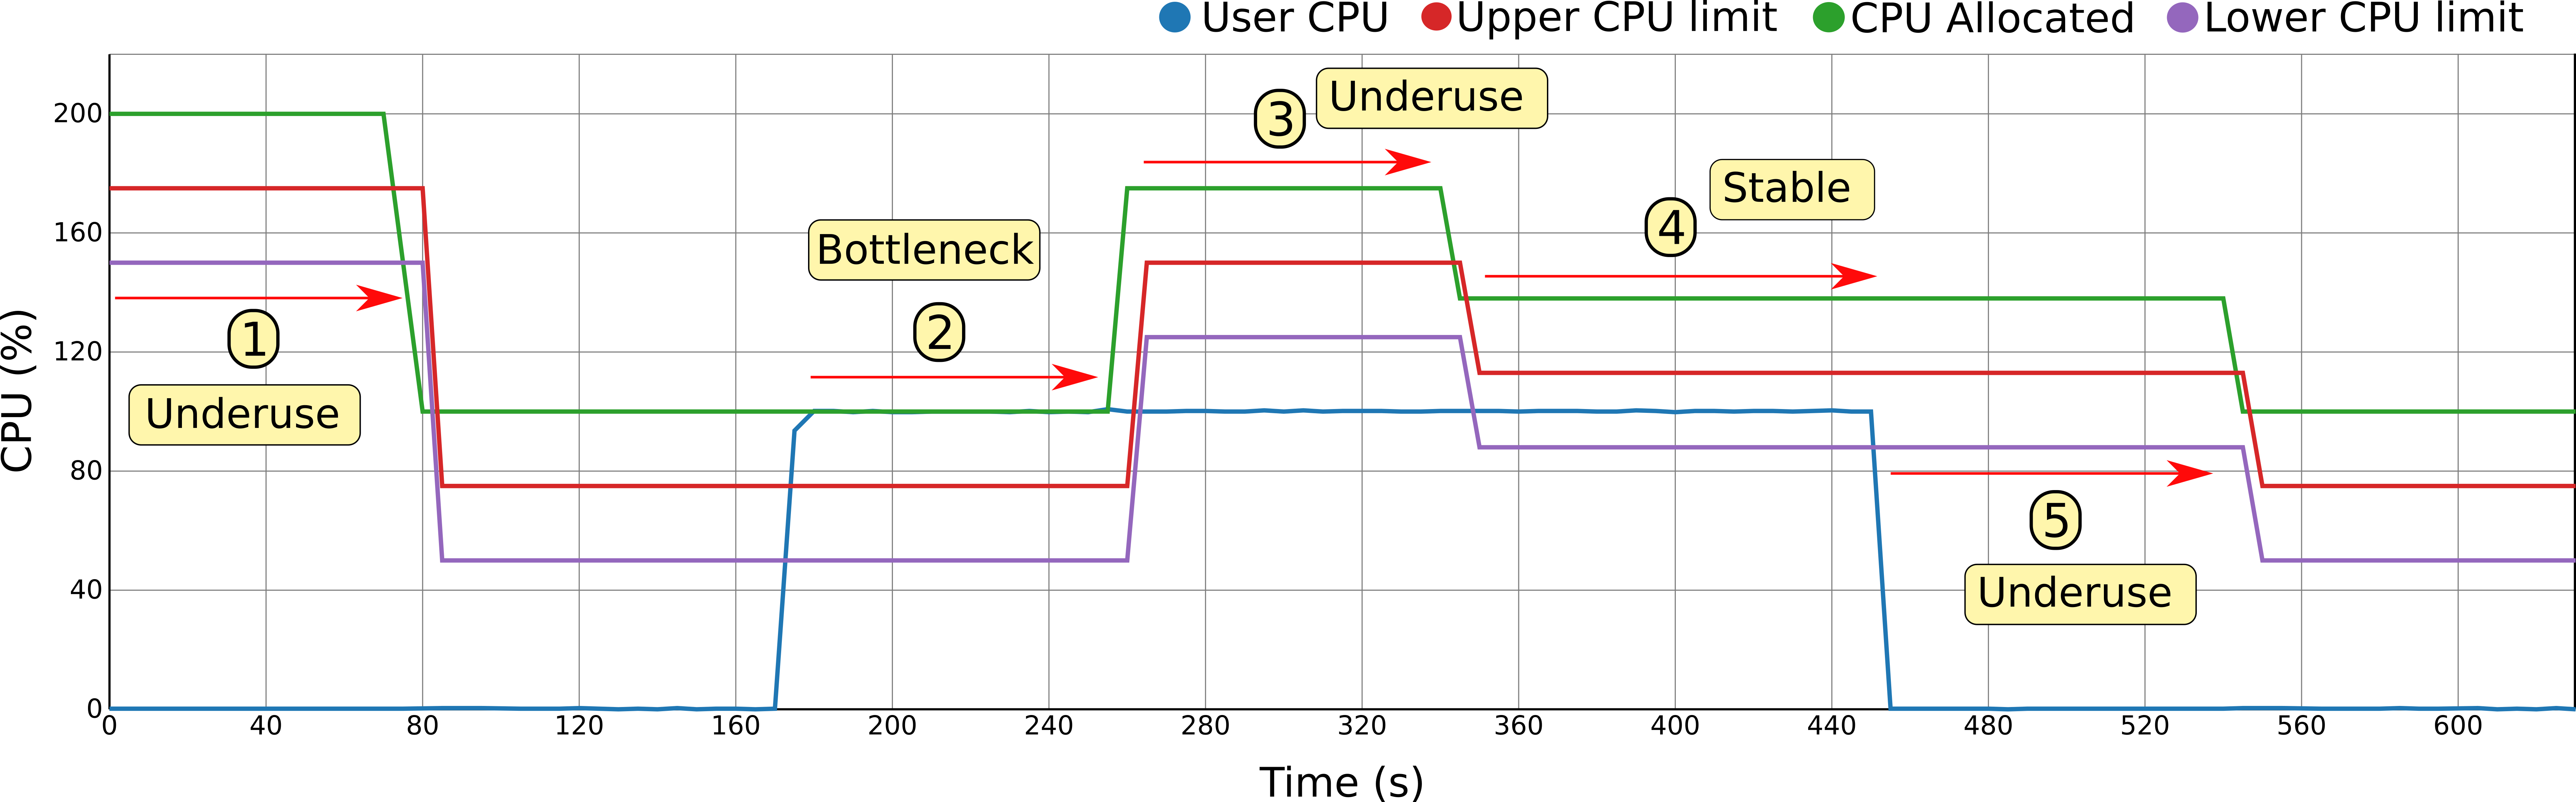
\includegraphics[width=0.99\textwidth]{../img/quickstart/scaling_examples.png}
	\caption{Examples of container scaling operations on a serverless environment}
	\label{fig:ContainerScalingExample}
\end{figure}


The behavior exposed on the image can be configured and tuned with a few, critical parameters, as explained on the Configuration Section~\ref{sec:Configuration}.

\subsection{Returning the containers to traditional instances}

If at any moment we want to stop the scaling from taking place for these containers, we have only to configure the containers to be left alone (unguarded): \newline

\noindent \code{bash scripts/Orchestrator/Structures/set\_to\_unguarded.sh cont0} \newline
\code{bash scripts/Orchestrator/Structures/set\_to\_unguarded.sh cont1} \newline

If at this point we consider that the resource limits are too low, we can always reset them.

\subsection{Shutting everything down}

In order to shut everything down we only have to stop the Python programs running the microservices.

However, it has to be noted that it is possible to implement a `partial' shut down of the system by only stopping the active services. Even further, the system can be inactivated by only stopping or de-activating the \textit{Scaler} microservice, something that we effectively did at the end of the Starting the services subsection.

\subsection{Orchestrator's API}
\begin{itemize}
\item \code{/service/ ['GET']}
\item \code{/service/<service\_name> ['GET', 'PUT']}
\item \code{/service/<service\_name>/<key> ['PUT']}
\item \code{/rule/ ['GET']}
\item \code{/rule/<rule\_name> ['GET']}
\item \code{/rule/<rule\_name>/activate ['PUT']}
\item \code{/rule/<rule\_name>/deactivate ['PUT']}
\item \code{/structure/ ['GET']}
\item \code{/structure/<structure\_name> ['GET']}
\item \code{/structure/<structure\_name>/resources ['GET']}
\item \code{/structure/<structure\_name>/resources/<resource> ['GET']}
\item \code{/structure/<structure\_name>/resources/<resource>/<parameter> ['GET', 'PUT']}
\item \code{/structure/<structure\_name>/guard ['PUT']}
\item \code{/structure/<structure\_name>/unguard ['PUT']}
\item \code{/structure/<structure\_name>/resources/<resource>/guard ['PUT']}
\item \code{/structure/<structure\_name>/resources/<resource>/unguard ['PUT']}
\item \code{/structure/<structure\_name>/resources/guard ['PUT']}
\item \code{/structure/<structure\_name>/resources/unguard ['PUT']}
\item \code{/structure/<structure\_name>/limits ['GET']}
\item \code{/structure/<structure\_name>/limits/<resource> ['GET']}
\item \code{/structure/<structure\_name>/limits/<resource>/boundary ['PUT']}
\item \code{/structure/<structure\_name>/guard\_policy/serverless ['PUT']}
\item \code{/structure/<structure\_name>/guard\_policy/fixed ['PUT']}
\item \code{/heartbeat ['GET']}
\end{itemize}


\section{Configuration}
\label{sec:Configuration}
The behavior of the \textit{\textbf{Serverless Container framework}} can be configured to better adapt to the needs of the applications. Such configuration can be even changed dynamically if needed thanks to the design choices.

The configuration can be divided between two dimensions, being the first the time dimension and the second one the resource limit dimension. To better approach these two dimensions, the first one is referred to as the Responsiveness of the framework, while the second one is referred to as the Benevolence.

\begin{figure}[!tb]
	\centering
	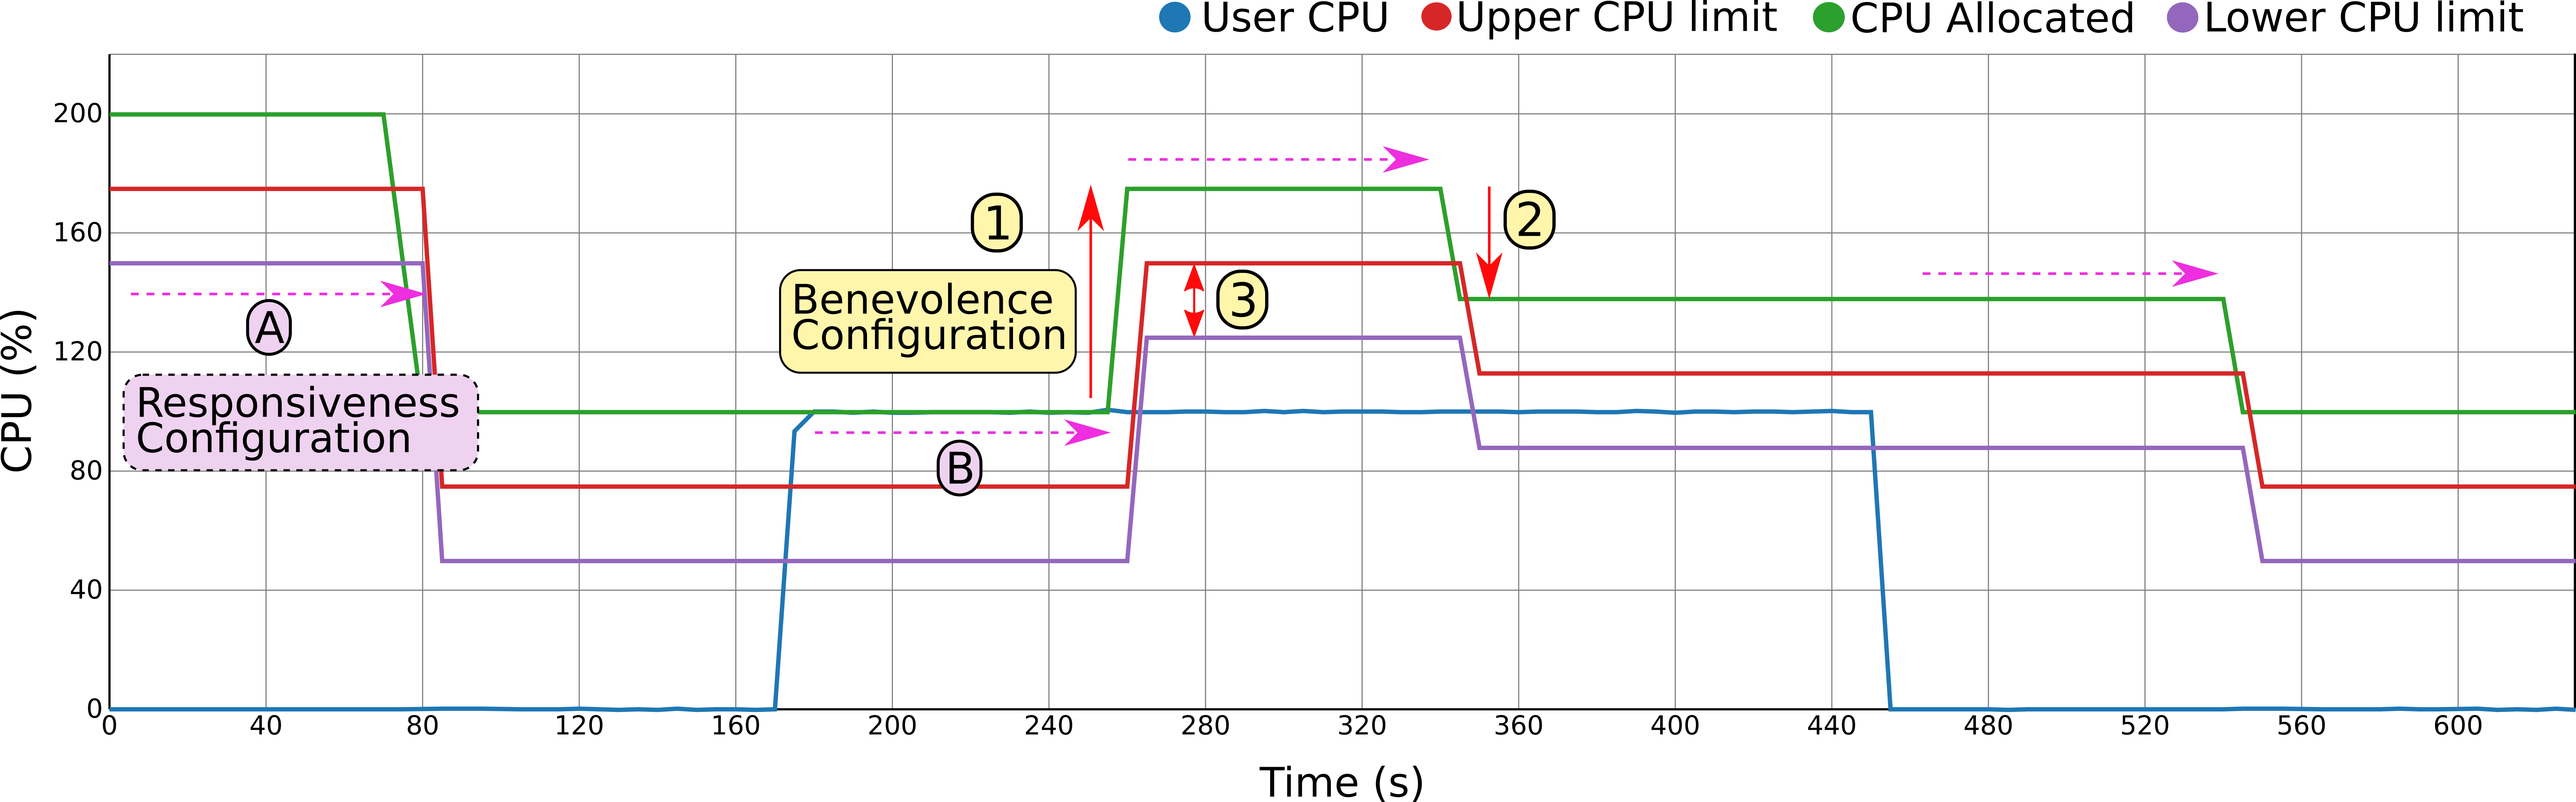
\includegraphics[width=0.99\textwidth]{../img/configuration/configuration.png}
	\caption{Configuration}
	\label{fig:Configuration}
\end{figure}

\subsection{Responsiveness}
As its name implies, this configuration aspect of the framework dictates how fast the changes are made when it comes to adapting the resource limits to the application's real usage. The reason why we have to take into account this, instead of just performing instant scaling operations once the limits have been surpassed, lies behind the concept of hysteresis.

If we consider hysteresis as the degree of variation of the resource usage patterns, we need to take into account some kind of time buffer before changing the resource limits. This time buffer allows to have some assurance that after a scaling operation, another one won't be needed soon after.

As seen on Figure~\ref{fig:ResponsivenessConfiguration}, the responsiveness can be modulated differently to adapt to two possible scenarios:
\begin{itemize}
	\item \textbf{A}: Time to pass before performing a scaling down operation.
	\item \textbf{B}: Time to pass before performing a scaling up operation.
\end{itemize}

It has to be noted the difference between the two. While on the A scenario we can allow more time to pass, as the resources are in the end being underutilized (the application is not being penalized), on the B scenario the application may be close to, or suffering a bottleneck, thus we may consider to shorten such times to avoid execution overheads.

\begin{figure}[!tb]
	\centering
	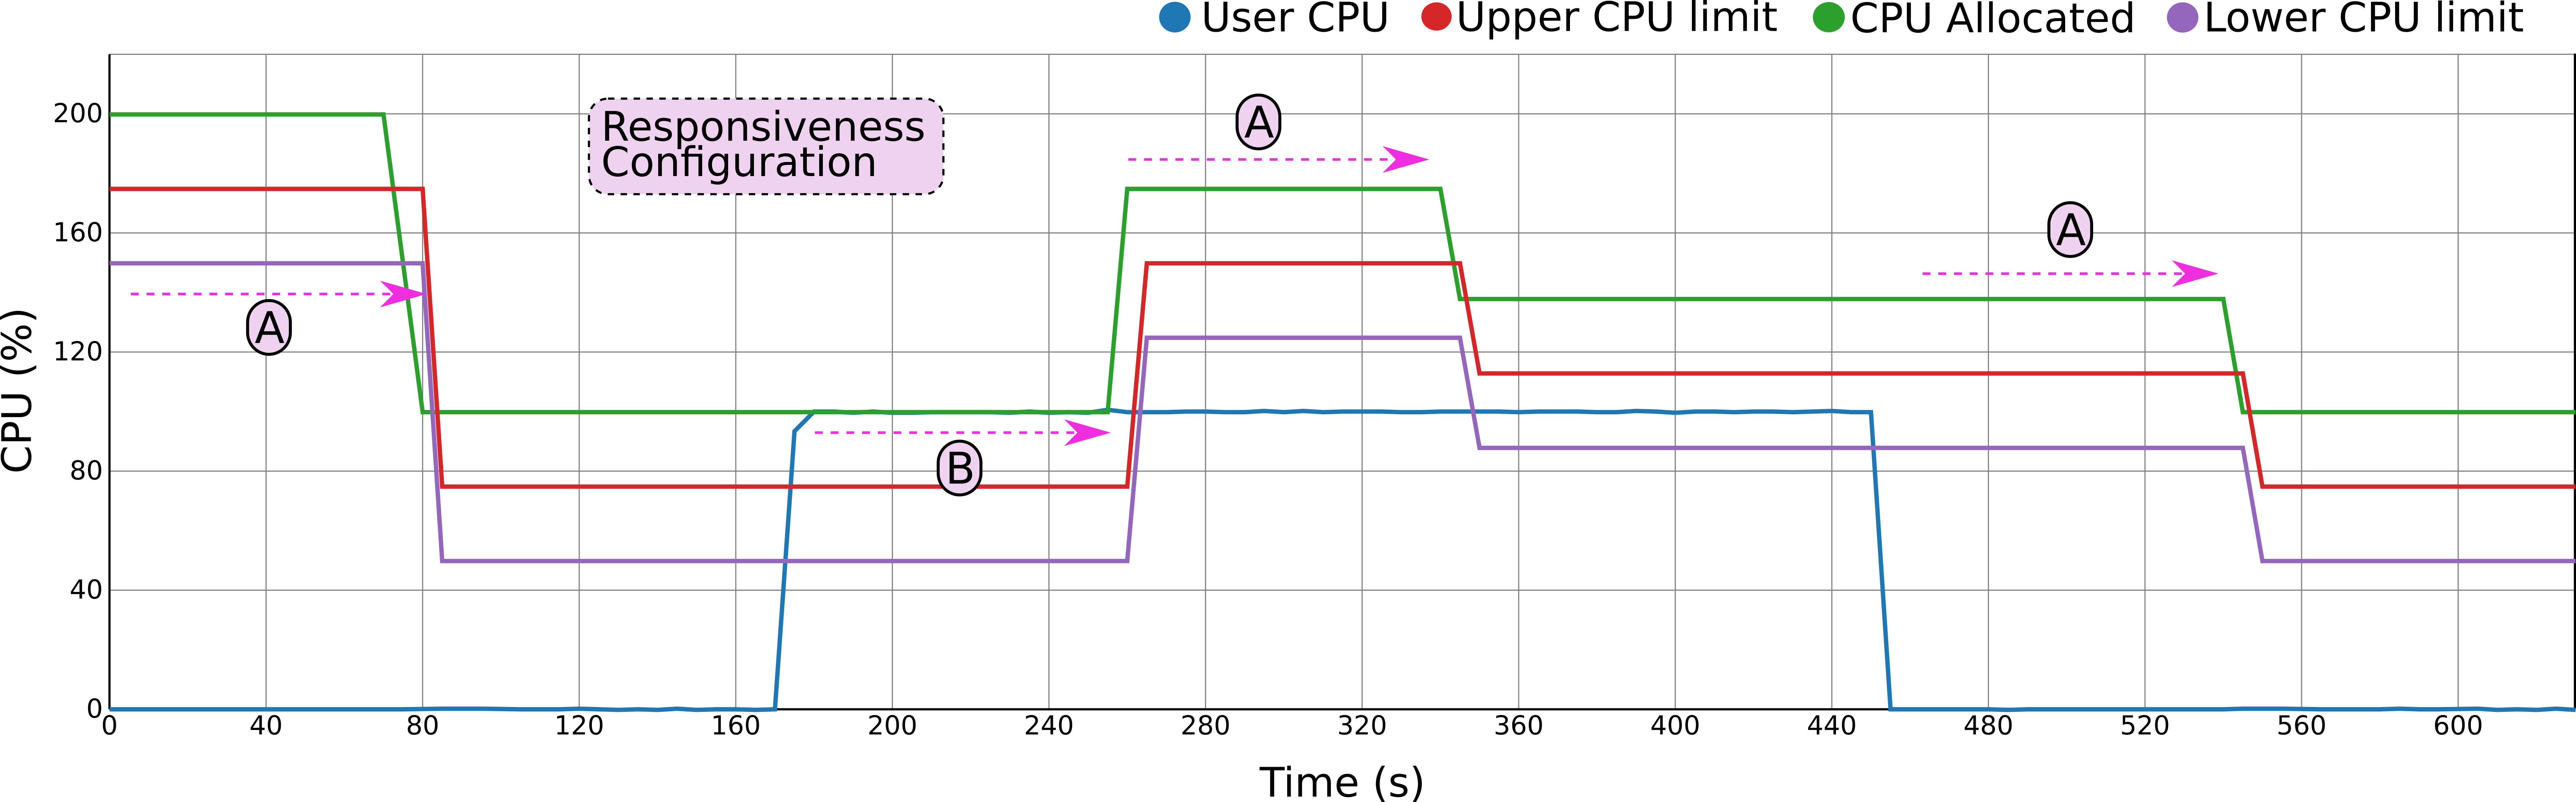
\includegraphics[width=0.99\textwidth]{../img/configuration/configuration_responsiveness.png}
	\caption{Responsiveness Configuration}
	\label{fig:ResponsivenessConfiguration}
\end{figure}

To tune the Responsiveness of the framework, the request-generating Rules will have to be modified.

\subsection{Benevolence}

In the case of Benevolence, as its name says, it modules how the framework addresses the scaling operations in terms of the number of resources that it takes away or that it gives. On the one hand, a `benevolent' framework adjusts the resources leaving an ample margin between the limits so that the areas are large enough to accommodate any resource variations, while at the same time giving a large number of resources when scaling up. On the other hand, if we want to push the serverless scenario to the limit we can set narrower boundaries and more restrained scaling up operations.

As seen in Figure~\ref{fig:BenevolenceConfiguration}, to module the behavior between these two options, thus tuning the framework to behave closer to the traditional instance or closer to the serverless paradigm, we can use the following configuration parameters:
\begin{itemize}
	\item \textbf{1) Scaling up amount}. A fixed and configurable amount.
	\item \textbf{2) Scaling down policy}. Although several are possible, to implement the serverless scenario the only one usable is the `fit to usage', which looks to set resource limits so that the usage falls between the upper and lower boundaries (stable area).
	\item \textbf{3) Boundary amount}. This parameter is used combined with the scaling down policy to define the final allocated resource limit.
\end{itemize}

To tune the Benevolence of the framework, mainly the amount parameter of the down-scaling Rules will have to be adapted.

\begin{figure}[!tb]
	\centering
	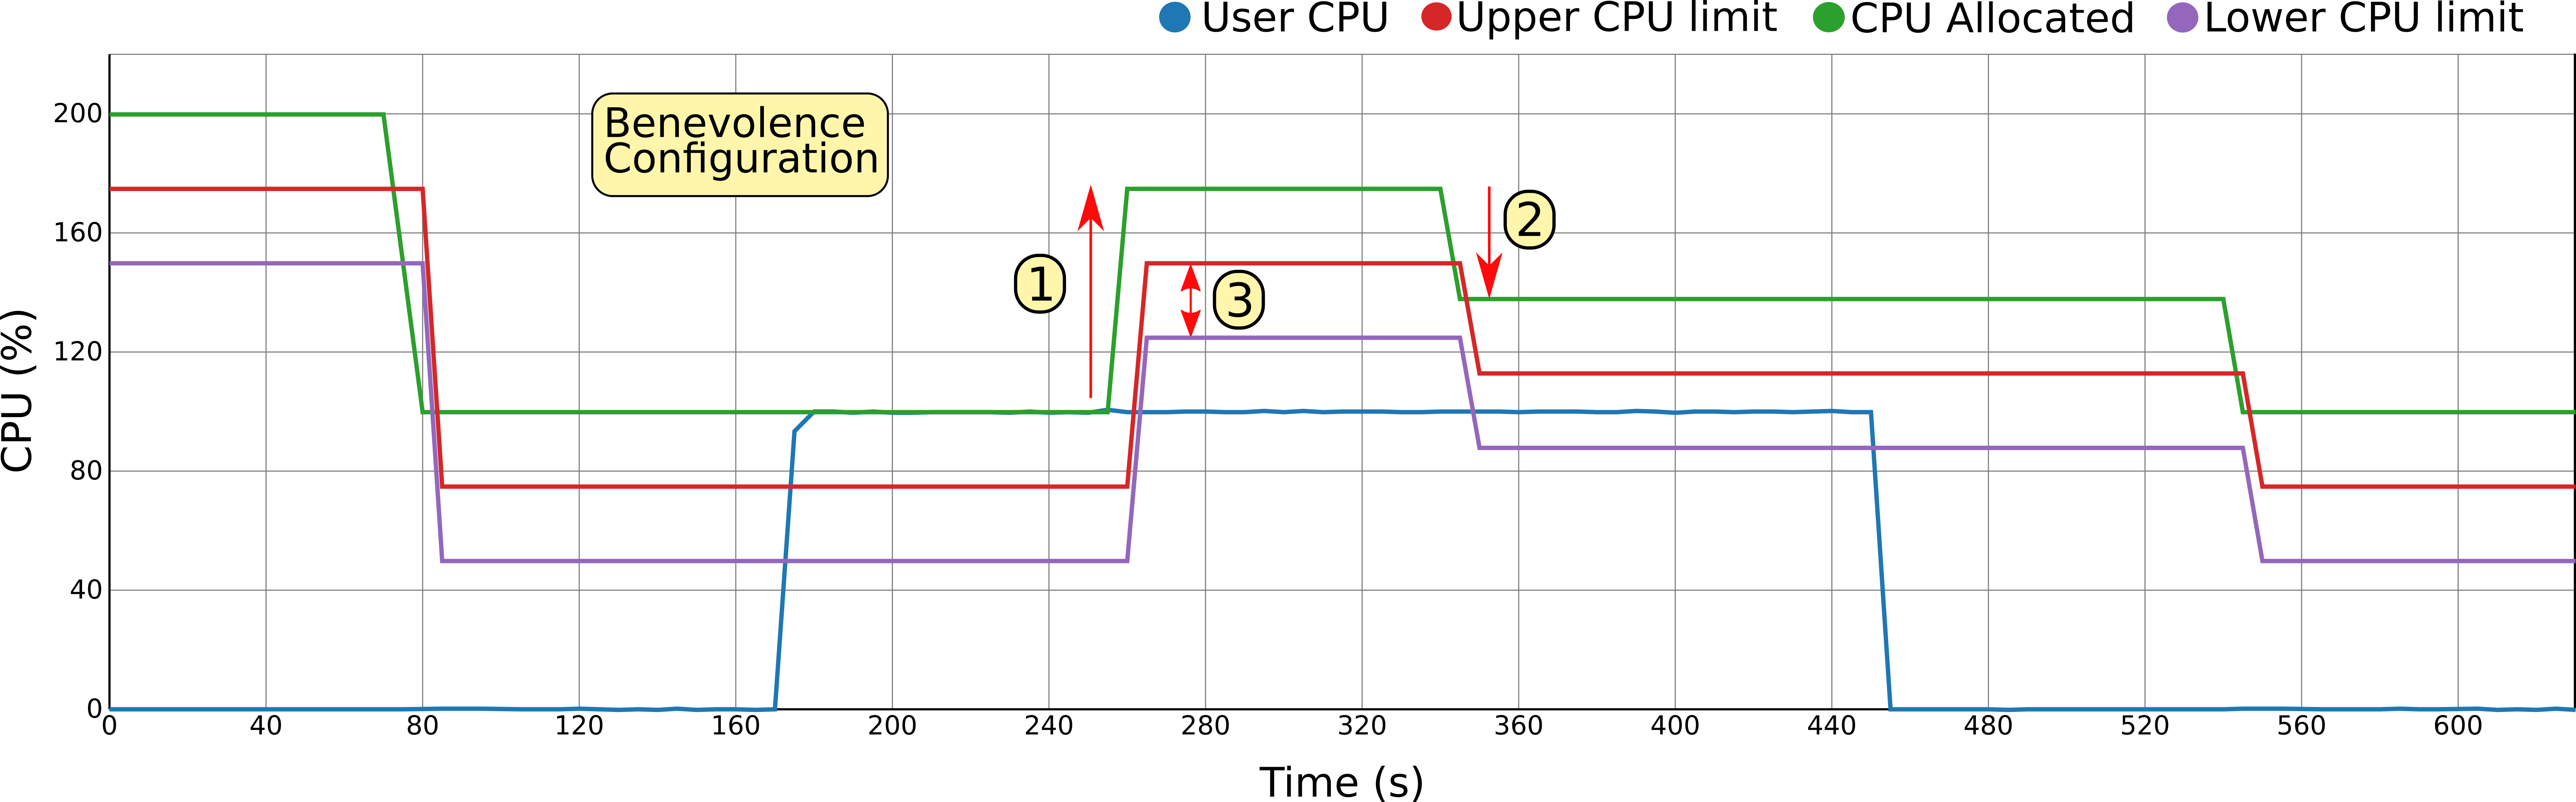
\includegraphics[width=0.99\textwidth]{../img/configuration/configuration_benevolence.png}
	\caption{Benevolence Configuration}
	\label{fig:BenevolenceConfiguration}
\end{figure}

\subsection{Rule Configuration}

As previously stated, in order to configure the framework on the vertical and time dimensions, the Rule documents have to be modified. 

To tune the Responsiveness, we have to modify the request-generating Rules to specify the amount of time windows desired before a scaling request is generated by the \textit{Guardian}. As seen in the Rule document of Listing~\ref{lst:Rule}, the number of time windows where the usage had to surpass the upper limits before one of this kind of requests is generated is 4. We can also notice that the number of the opposite event (usage fell below the lower limit) must also be lower than 2. This is done in order to avoid hysteresis, skipping scenarios where the resource usage is highly volatile and constantly crossing both limits.

\begin{center}
	\lstset{basicstyle=\footnotesize}
	\lstset{linewidth=1\textwidth}
	\lstset{language=perl}
	\lstset{xleftmargin=0.0725\textwidth}
	\lstset{showstringspaces=false}
	\lstset{backgroundcolor=\color{backcolour}}
	\lstset{captionpos=b}
	\lstset{numbers=left}
	\lstset{tabsize=1}
	\begin{lstlisting}[float=bt,frame=bt,caption=Example of a Limit document,label=lst:Rule]
	CpuRescaleUp = dict(
		_id='CpuRescaleUp',
		type='rule',
		resource="cpu",
		name='CpuRescaleUp',
		rule=dict(
			{"and": [
				{">=": [
					{"var": "events.scale.up"},
					4]},
				{"<=": [
					{"var": "events.scale.down"},
					2]}
			]}),
		events_to_remove=4,
		generates="requests",
		action={"requests": ["CpuRescaleUp"]},
		amount=75,
		rescale_by="amount",
		active=True
	)
	\end{lstlisting}
\end{center}

When it comes to Benevolence, we can also see on the Rule document in Listing~\ref{lst:Rule} that the amount of CPU increased on a scaling up operation will be 75 shares (i.e., three-quarters of a core).

Finally, in order to configure the boundary parameter, we have to use the Limits documents of each container. On these documents there is a boundary applied for each resource, as seen in Listing~\ref{lst:Limit}.

\begin{center}
	\lstset{basicstyle=\footnotesize}
	\lstset{linewidth=1\textwidth}
	\lstset{language=perl}
	\lstset{xleftmargin=0.0725\textwidth}
	\lstset{showstringspaces=false}
	\lstset{backgroundcolor=\color{backcolour}}
	\lstset{captionpos=b}
	\lstset{numbers=left}
	\lstset{tabsize=1}
	\begin{lstlisting}[float=bt,frame=bt,caption=Example of a Limit document,label=lst:Limit]
cpu: {
	boundary: 25,
	lower: 50,
	upper: 75
	}
}
	\end{lstlisting}
\end{center}


\subsection{Service Configuration}

As previously stated, most of the microservices work with polling time windows. The relation between all of the services' time windows may be important, although the framework has been designed to be robust and tend for a behavior akin to an eventual consistency. Figure~\ref{fig:TimeWindowAnalysis} describes such relationships.

\begin{figure}[!tb]
	\centering
	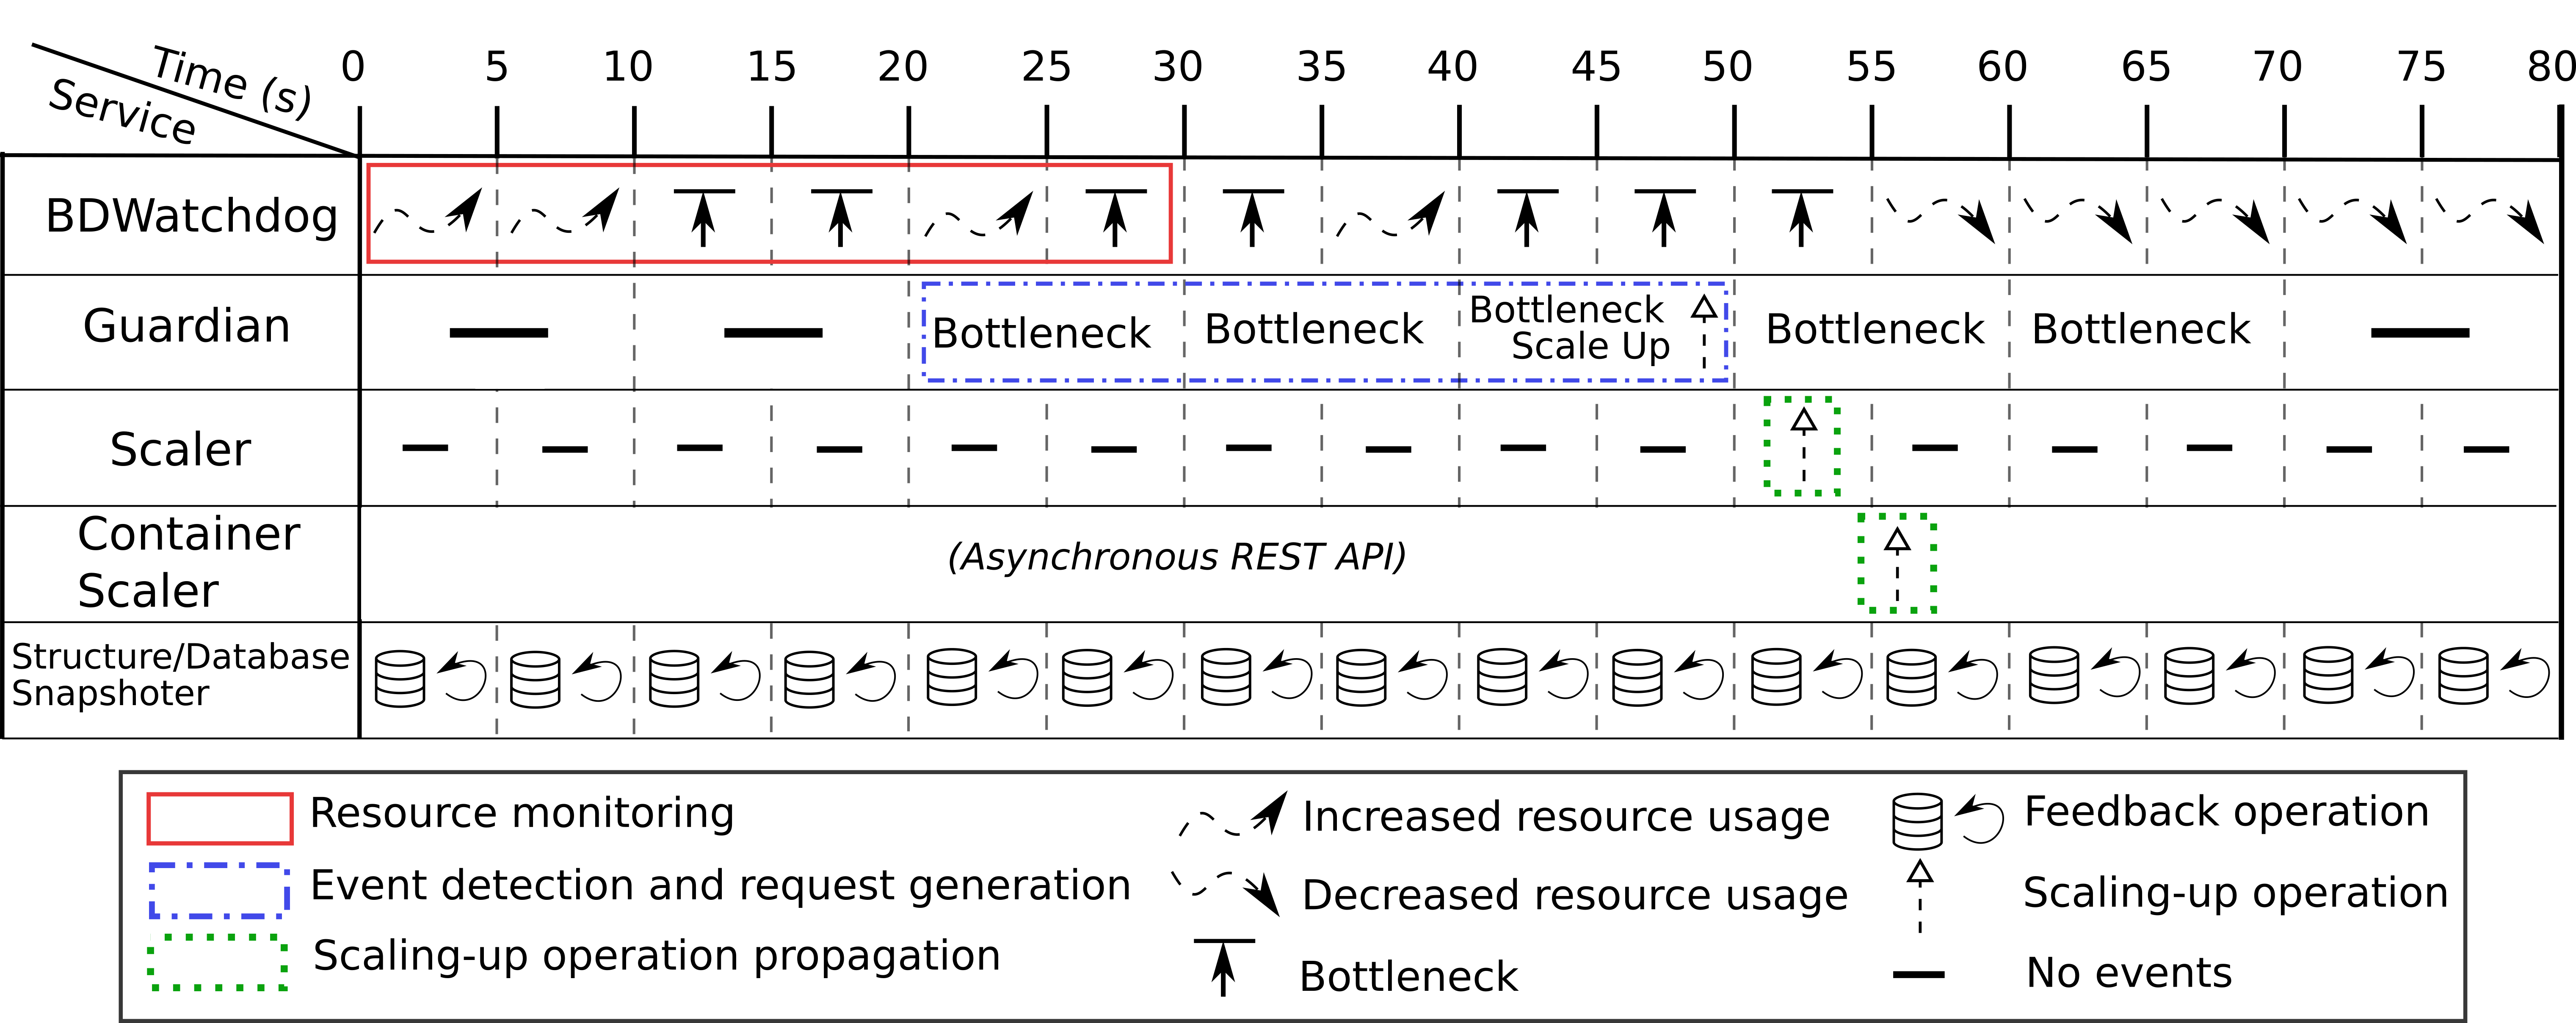
\includegraphics[width=0.99\textwidth]{../img/configuration/time_window_analysis.png}
	\caption{Time window analysis}
	\label{fig:TimeWindowAnalysis}
\end{figure}

Nevertheless, both the \textit{Guardian} and the \textit{Scaler} time window configuration may be worth mentioning:
\begin{itemize}
	\item \textbf{\textit{Guardian}} : In this case, the time window directly influences the Responsiveness of the framework, as previously seen the scaling operations are performed by measuring the number of time windows that the resource usage spends on one specific scenario.
	\item \textbf{\textit{Scaler}} : When it comes to the \textit{Scaler} service, it is important that its polling time window is lower than the \textit{Guardian} service one, as otherwise the Requests could be applied in an unordered fashion.
\end{itemize}

\section{Contact}

\textit{\textbf{Serverless Containers}} has been entirely developed in the \href{http://gac.udc.es/english/}{Computer Architecture Group} at the \href{https://www.udc.es/index.html?language=en}{University of A Coru\~na} by the following authors:

\begin{itemize}
	\item Jonatan Enes Alvarez \url{http://gac.udc.es/~jonatan.enes/}
	\item Roberto R. Exp\'osito: \url{http:gac.udc.es/~rreye}
	\item Juan Touri\~no: \url{http:gac.udc.es/~juan}
\end{itemize}

For any question regarding the \textit{\textbf{Serverless Containers framework}}, whether about the source code, its usage or functionalities, please address via email to Jonatan Enes (jonatan.enes@udc.es).

\addcontentsline{toc}{chapter}{References}
\bibliography{manual}
\bibliographystyle{plain}

\end{document}
